% concatenated from long.tex, preamble.tex, introduction.tex, easy.tex, girth3.tex, girth4.tex, tree.tex

\documentclass[a4paper,UKenglish,cleveref, autoref, thm-restate]{lipics-v2021}
%This is a template for producing LIPIcs articles. 
%See lipics-v2021-authors-guidelines.pdf for further information.
%for A4 paper format use option "a4paper", for US-letter use option "letterpaper"
%for british hyphenation rules use option "UKenglish", for american hyphenation rules use option "USenglish"
%for section-numbered lemmas etc., use "numberwithinsect"
%for enabling cleveref support, use "cleveref"
%for enabling autoref support, use "autoref"
%for anonymousing the authors (e.g. for double-blind review), add "anonymous"
%for enabling thm-restate support, use "thm-restate"
%for enabling a two-column layout for the author/affilation part (only applicable for > 6 authors), use "authorcolumns"
%for producing a PDF according the PDF/A standard, add "pdfa"

%\pdfoutput=1 %uncomment to ensure pdflatex processing (mandatatory e.g. to submit to arXiv)
%\hideLIPIcs  %uncomment to remove references to LIPIcs series (logo, DOI, ...), e.g. when preparing a pre-final version to be uploaded to arXiv or another public repository

%\graphicspath{{./graphics/}}%helpful if your graphic files are in another directory
\usepackage[utf8]{inputenc}
\usepackage{tikz,amsmath,amssymb,amsthm}
%\usepackage[shortlabels]{enumitem}
\usepackage{color,url}
\usepackage{hyperref}
\usepackage[capitalise]{cleveref}
\usepackage{xspace}
\usepackage{todonotes}
\usepackage{thm-restate}
\usepackage{comment}
\usepackage{thmtools}

%%%% Theorems
%\theoremstyle{plain}
%\newtheorem{theorem}{Theorem}
%\newtheorem{lemma}{Lemma}
%\newtheorem{observation}{Observation}
%\newtheorem{corollary}{Corollary}
%\newtheorem{proposition}{Proposition}
%\newtheorem{conjecture}[theorem]{Conjecture}
%\newtheorem{question}[theorem]{Question}
%\newtheorem{definition}[theorem]{Definition}
%\newtheorem{claim}{Claim}[theorem]
%\newenvironment{claimproof}{\noindent\textit{Proof of Claim \theclaim:}}{\hfill$\lrcorner$} 
%\theoremstyle{plain}
\newtheorem{fact}{Fact}

\newcommand{\pname}[1]{\textnormal{\textsc{#1}}}
\newcommand{\cclass}[1]{\textnormal{\textsf{#1}}}
\newcommand{\VC}{\pname{Vertex Cover}}
\newcommand{\NPC}{NP-complete}
\newcommand{\HFD}{\pname{$H$-free Edge Deletion}}
\newcommand{\PTFD}{\pname{$P_3$-free Edge Deletion}}
\newcommand{\PFFD}{\pname{$P_4$-free Edge Deletion}}
\newcommand{\PSD}{\pname{$\Pi$ Subdivision}}
\newcommand{\HFS}{\pname{$H$-free Subdivision}}
\newcommand{\SHFS}{\pname{$\mathcal{H}$-free Subdivision}}
\newcommand{\HDFS}{\pname{$H'$-free Subdivision}}
\newcommand{\sandeep}[1]{\textcolor{orange}{S:#1}}

\newcommand{\N}{\mathbb{N}}
\newcommand{\girth}{\mathrm{girth}}
\newcommand{\cH}{\mathcal{H}}
\newcommand{\tH}{\widetilde{H}}
\newcommand{\dist}{\mathrm{dist}}
\newcommand{\core}{\mathrm{core}}
\newcommand{\tc}{\widetilde{c}}

%\usepackage[subtle]{savetrees}
%\usepackage{geometry}
%\usepackage{tikz,amsmath, amssymb,bm,color, amsthm}
%\usetikzlibrary{positioning, calc,chains,fit,shapes,decorations.pathmorphing}
%\usetikzlibrary{circuits.logic.US,circuits.logic.IEC,fit}
%\usepackage{enumerate}
%\usepackage{comment}
%\usepackage{tikz}
%\usepackage{graphics}
%\usepackage[cm]{fullpage}
%\usepackage{longtable}
%\usepackage{mdframed}
%\usepackage{caption}
%\usepackage{subcaption}
%\usepackage{slashbox}
%\usepackage{url}
%\usepackage{framed}
%\usepackage{array}
%\usepackage{tabu}
%\usepackage{lscape}
%\usepackage{multirow}
%\usepackage{ulem}
%\usepackage{multicol}
%\usepackage{placeins}
%\usepackage{cite}
%\usepackage{enumerate}

%\usetikzlibrary{positioning,chains,shapes,calc}
%\usetikzlibrary{fit}
%\thispagestyle{empty}
%\usetikzlibrary{
%  graphs,
%  graphs.standard
%}

%\usepackage[shortlabels]{enumitem}
%\usepackage{comment}
%\setlistdepth{9}

%\newlist{myEnumerate}{enumerate}{9}
%\setlist[myEnumerate,1]{label=(\arabic*)}
%\setlist[myEnumerate,2]{label=(\Roman*)}
%\setlist[myEnumerate,3]{label=(\Alph*)}
%\setlist[myEnumerate,4]{label=(\roman*)}
%\setlist[myEnumerate,5]{label=(\alph*)}
%\setlist[myEnumerate,6]{label=(\arabic*)}
%\setlist[myEnumerate,7]{label=(\Roman*)}
%\setlist[myEnumerate,8]{label=(\Alph*)}
%\setlist[myEnumerate,9]{label=(\roman*)}


\bibliographystyle{plainurl}% the mandatory bibstyle

\title{On the complexity of edge subdivision to $H$-free graphs} %TODO Please add

%\titlerunning{Dummy short title} %TODO optional, please use if title is longer than one line
\author{Marta Piecyk}{CISPA Helmholtz Center for Information Security, Germany}{marta.piecyk@cispa.de}{0000-0001-9162-8300}{}

\author{R. B. Sandeep}{Indian Institute of Technology Dharwad, India}{sandeeprb@iitdh.ac.in}{0000-0003-4383-1819}{Supported by Anusandhan National Research Foundation (India) grant MTR/2022/000692}%TODO mandatory, please use full name; only 1 author per \author macro; first two parameters are mandatory, other parameters can be empty. Please provide at least the name of the affiliation and the country. The full address is optional. Use additional curly braces to indicate the correct name splitting when the last name consists of multiple name parts.


\authorrunning{M. Piecyk and R.\,B. Sandeep} %TODO mandatory. First: Use abbreviated first/middle names. Second (only in severe cases): Use first author plus 'et al.'

\Copyright{Marta Piecyk and R. B. Sandeep} %TODO mandatory, please use full first names. LIPIcs license is "CC-BY";  http://creativecommons.org/licenses/by/3.0/

%\ccsdesc[100]{\textcolor{red}{Replace ccsdesc macro with valid one}} %TODO mandatory: Please choose ACM 2012 classifications from https://dl.acm.org/ccs/ccs_flat.cfm 
\ccsdesc[500]{Theory of computation~Graph algorithms analysis}
\ccsdesc[500]{Theory of computation~Problems, reductions and completeness}
\ccsdesc[300]{Theory of computation~Parameterized complexity and exact algorithms}

\keywords{Edge subdivision, $H$-free graphs, Parameterized lower bound} %TODO mandatory; please add comma-separated list of keywords

\category{} %optional, e.g. invited paper

\relatedversion{} %optional, e.g. full version hosted on arXiv, HAL, or other respository/website
%\relatedversiondetails[linktext={opt. text shown instead of the URL}, cite=DBLP:books/mk/GrayR93]{Classification (e.g. Full Version, Extended Version, Previous Version}{URL to related version} %linktext and cite are optional

%\supplement{}%optional, e.g. related research data, source code, ... hosted on a repository like zenodo, figshare, GitHub, ...
%\supplementdetails[linktext={opt. text shown instead of the URL}, cite=DBLP:books/mk/GrayR93, subcategory={Description, Subcategory}, swhid={Software Heritage Identifier}]{General Classification (e.g. Software, Dataset, Model, ...)}{URL to related version} %linktext, cite, and subcategory are optional

%\funding{(Optional) general funding statement \dots}%optional, to capture a funding statement, which applies to all authors. Please enter author specific funding statements as fifth argument of the \author macro.

\acknowledgements{The project was initiated at STRUG: Structural Graph Theory Bootcamp, funded by the ``Excellence initiative – research university (2020–2026)'' of University of Warsaw. We are grateful to Erik Jan van Leeuwen for stimulating discussions on the topic.}%optional

\nolinenumbers %uncomment to disable line numbering



%Editor-only macros:: begin (do not touch as author)%%%%%%%%%%%%%%%%%%%%%%%%%%%%%%%%%%
\EventEditors{John Q. Open and Joan R. Access}
\EventNoEds{2}
\EventLongTitle{42nd Conference on Very Important Topics (CVIT 2016)}
\EventShortTitle{CVIT 2016}
\EventAcronym{CVIT}
\EventYear{2016}
\EventDate{December 24--27, 2016}
\EventLocation{Little Whinging, United Kingdom}
\EventLogo{}
\SeriesVolume{42}
\ArticleNo{23}
%%%%%%%%%%%%%%%%%%%%%%%%%%%%%%%%%%%%%%%%%%%%%%%%%%%%%%

\begin{document}

\maketitle

%TODO mandatory: add short abstract of the document
\begin{abstract}
Subdividing an edge $uv$ in a graph $G$ is the operation in which the edge $uv$ is deleted, and a new vertex $w$ together with two edges $uw$ and $vw$ is introduced. A $k$-subdivision of a graph $G$ is a graph obtained from $G$ by applying $k$ subdivisions successively. For a graph $H$, the \textsc{$H$-free Subdivision} problem is defined as follows: given a graph $G$ and an integer $k$, decide whether $G$ can be transformed into a graph without any induced copy of $H$ by performing at most $k$ edge subdivisions.

We first observe that if $H$ is a subdivided star, that is, a tree with at most one vertex of degree at least $3$, or a subdivided bistar, that is, a tree with exactly two adjacent vertices of degree at least $3$, then the problem is trivially solvable in polynomial time. This observation can be easily extended to show that if every component of $H$ is either a subdivided star or a subdivided bistar, and at most one component of $H$ is a subdivided bistar, then \textsc{$H$-free Subdivision} is polynomial-time solvable.

On the negative side, we prove that \textsc{$H$-free Subdivision} is NP-complete and, assuming the Exponential Time Hypothesis, cannot be solved in time $2^{o(k)}\cdot n^{O(1)}$ if $H$ satisfies any of the following properties:
\begin{itemize}
    \item $H$ has minimum degree at least $2$, and the neighborhood of every degree-$2$ vertex induces a $K_2$;
    \item the vertices of degree at least $3$ in $H$ induce a graph with at least two edges;
    \item $H$ has a triangle with two vertices of degree at least $3$;
    \item $H$ contains, as an induced subgraph, the $6$-vertex graph obtained from two vertex-disjoint triangles by adding an edge between them;
    \item $H$ contains exactly one triangle;
    \item $H$ has girth at least $4$;
    \item $H$ is a tree with exactly two vertices of degree at least $3$ which are at distance $2$ or at least $4$.
\end{itemize}
A simple bounded search-tree algorithm gives a
$2^{O(k)}\cdot n^{O(1)}$-time fixed-parameter tractable algorithm for the problem.
Our lower bound shows that, for the cases in which we prove hardness, this running time cannot be substantially improved, assuming the Exponential Time Hypothesis.

\end{abstract}



\newpage
\section{Introduction}

A typical graph modification problem is characterized by one or more graph operations and a target graph class.
The input consists of a graph and a budget, and the objective is to decide whether the graph can be transformed into a graph belonging to the target class by applying the operation or operations within the given budget.
Many well-known computational graph problems, such as \textsc{Vertex Cover} and \textsc{Feedback Vertex/Arc Set}, can be stated as graph modification problems.

We initiate the computational study of graph modification problems based on a very familiar graph operation: edge subdivision.
An edge subdivision of an edge $uv$ of a graph $G$ is the operation that removes the edge $uv$, adds a new vertex $w$, and adds the two edges $uw$ and $wv$.
A $k$-subdivision of $G$ is a graph obtained from $G$ by applying $k$ edge subdivisions successively.
For a graph class or property $\Pi$, we consider the following problem.

\medskip
\noindent
\textsc{$\Pi$-Subdivision}: Given a graph $G$ and an integer $k$, decide whether $G$ can be transformed into a graph with property $\Pi$ by applying at most $k$ edge subdivisions.

\medskip
It is easy to observe that edge subdivisions do not destroy minors of the input graph.
Therefore, \textsc{$\Pi$-Subdivision} is trivial when $\Pi$ is a minor-closed graph class, such as the class of planar graphs or the class of forests: if the input graph contains a forbidden minor for $\Pi$, then it is a no-instance, and otherwise it is a yes-instance.
The same argument applies to induced-minor-closed graph classes, such as the class of chordal graphs.

A hereditary graph class is a graph class closed under vertex deletion.
It is well known that every hereditary graph class can be characterized by a (possibly infinite) set of forbidden induced subgraphs.
Hereditary graph classes are standard target classes for graph modification problems.
Thus, it is natural to consider the class of $H$-free graphs, that is, graphs with no induced copy of a fixed graph $H$, as a target class.
Indeed, such classes have been studied as target classes for a wide range of graph modification problems; see Table~\ref{tab:complexity-summary}.

\begin{table}[ht]
\centering
\begin{tabular}{|c|p{4cm}|p{4cm}|}
\hline
\textbf{Operation} & \textbf{P} & \textbf{NP-complete} \\
\hline
vertex deletion
& $H=K_1$~[trivial]
& otherwise~\cite{yannakakis1978node} \\
\hline
edge deletion
& $|E(H)|\leq 1$~[trivial]
& otherwise~\cite{DBLP:journals/siamdm/AravindSS17} \\
\hline
edge completion
& at most 1 nonedge~[trivial]
& otherwise~\cite{DBLP:journals/siamdm/AravindSS17} \\
\hline
edge editing
& $|V(H)|\leq 2$~[trivial]
& otherwise~\cite{DBLP:journals/siamdm/AravindSS17} \\
\hline
edge contraction
& $H\in\{K_1,K_2\}$~[trivial]
& otherwise~\cite{chakraborty2023contracting} \\
\hline
subgraph complementation
& paths on at most four vertices, complete graphs, paw~\cite{antony2022subgraph}
& $K_{1,t}$ for $t\geq 5$, $P_t$ and $C_t$ for $t\geq 7$, etc.~\cite{antony2022subgraph} \\
\hline
switching
& $|V(H)|\leq 2$, paw~\cite{antony2024switching}
& $P_t$ for $t\geq 10$, $C_t$ for $t\geq 7$, etc.~\cite{antony2024switching} \\
\hline
vertex splitting
& $|V(H)|\leq 2$, $K_1+K_2$~\cite{firbas2024complexity}
& $2$-connected graphs, etc.~\cite{firbas2024complexity} \\
\hline
\end{tabular}
\caption{Summary of complexity results on graph modification to $H$-free graphs.}
\label{tab:complexity-summary}
\end{table}

We study the complexity of the following problem.

\medskip
\noindent
\textsc{$H$-free Subdivision}: Given a graph $G$ and an integer $k$, decide whether $G$ can be transformed into an $H$-free graph by applying at most $k$ edge subdivisions.

\medskip
A \emph{star} is a connected graph with at most one vertex of degree at least $2$.
A \emph{bistar} is a connected graph with exactly two vertices of degree at least $3$, and these two vertices are adjacent, and all the remaining vertices have degree $1$.
A \emph{subdivided star} is a graph obtained from a star by subdividing its edges zero or more times. 
A \emph{subdivided bistar} is a graph obtained from a bistar by subdividing, zero or more times, only the edges other than the edge joining the two vertices of degree at least $3$.
It is easy to observe that an induced subdivided star cannot be destroyed by edge subdivisions, and the only way to destroy an induced subdivided bistar is to subdivide the edge joining its two vertices of degree at least $3$.
Thus we obtain our first observation.

\begin{observation}
\label{obs:poly}
Let $H$ be a graph such that every connected component of $H$ is either a subdivided star or a subdivided bistar, and at most one connected component of $H$ is a subdivided bistar.
Then \HFS\ is polynomial-time solvable.
\end{observation}

We conjecture that these are the only polynomial-time solvable cases.

\begin{conjecture}
\label{con:main}
\HFS\ is NP-complete if $H$ has at least two components that are subdivided bistars, or if $H$ has a component that is neither a subdivided star nor a subdivided bistar.
Furthermore, assuming the Exponential Time Hypothesis (ETH), the problem cannot be solved in time $2^{o(k)}\cdot n^{O(1)}$.
\end{conjecture}

In this paper, we verify \cref{con:main} for many graphs $H$.
We start with the following theorem.

\begin{restatable}{theorem}{EasyTheorem}
\label{thm:easy}
Let $H$ be a graph satisfying at least one of the following properties:
\begin{itemize}
    \item $H$ has minimum degree at least $2$, and the neighborhood of every degree-$2$ vertex induces a $K_2$;
    \item the vertices of degree at least $3$ induce a graph with at least two edges.
\end{itemize}
Then \textsc{$H$-free Subdivision} is NP-complete.
Furthermore, assuming the ETH, the problem cannot be solved in time
$2^{o(k)}\cdot n^{O(1)}$.
\end{restatable}

Next, we handle several graphs of girth $3$.
After excluding the cases covered by \cref{thm:easy}, the triangles containing vertices of degree at least $3$ have a very restricted structure.
We call a triangle a \emph{hanging triangle} if it contains exactly one vertex of degree at least $3$, and a \emph{roof triangle} if it contains exactly two vertices of degree at least $3$.
The vertices of degree at least $3$ in such a triangle are called its \emph{attachment vertices}.

\begin{restatable}{theorem}{GirthThreeTheorem}
\label{thm:girth3}
Let $H$ be a graph satisfying at least one of the following properties:
\begin{itemize}
    \item $H$ has a roof triangle;
    \item $H$ has two hanging triangles whose attachment vertices are adjacent.
\end{itemize}
Then \textsc{$H$-free Subdivision} is NP-complete.
Furthermore, assuming the ETH, the problem cannot be solved in time
$2^{o(k)}\cdot n^{O(1)}$.
\end{restatable}

We also prove that the same holds for graphs that contain precisely one triangle.

\begin{restatable}{theorem}{GirthUniqueTriangle}
\label{thm:girth3-Unique-Triangle}
Let $H$ be a graph that contains precisely one triangle.
Then \textsc{$H$-free Subdivision} is NP-complete.
Furthermore, assuming the ETH, the problem cannot be solved in time
$2^{o(k)}\cdot n^{O(1)}$.
\end{restatable}

Among graphs of girth $3$, the only graphs not covered by \cref{thm:easy}, \cref{thm:girth3}, and \cref{thm:girth3-Unique-Triangle} are those obtained from graphs of girth at least $4$ by attaching at least two hanging triangles in such a way that no two attachment vertices are adjacent.

We then completely verify the conjecture for non-forest graphs of girth at least $4$.

\begin{restatable}{theorem}{GirthFourTheorem}
\label{thm:girth-4}
Let $H$ be a graph which is not a forest and such that $\girth(H)\geq 4$.
Then \textsc{$H$-free Subdivision} is NP-complete.
Furthermore, assuming the ETH, the problem cannot be solved in time
$2^{o(k)}\cdot n^{O(1)}$.
\end{restatable}

Finally, we consider trees and obtain the following result, where a branching vertex is a vertex with degree at least 3.

\begin{restatable}{theorem}{TreeTheorem}
\label{thm:tree}
Let $H$ be a tree with exactly two branching vertices, and suppose that these two vertices are at distance $2$ or at least $4$.
Then \textsc{$H$-free Subdivision} is NP-complete.
Moreover, assuming the ETH, the problem cannot be solved in time
$2^{o(k)}\cdot n^{O(1)}$.
\end{restatable}
Note that, among trees with exactly two branching vertices, the cases not covered by \cref{thm:tree} are precisely those in which the branching vertices are at distance $1$ or $3$.
The former case corresponds to a subdivided bistar and is handled by \cref{obs:poly}.
For the latter case, we do not have a reduction that yields a parameterized subexponential-time lower bound under the ETH.

A simple bounded search-tree algorithm gives a
$2^{O(k)}\cdot n^{O(1)}$-time fixed-parameter tractable algorithm for the \textsc{$H$-free Subdivision} problem.
Our lower bound shows that, for the cases in which we prove hardness, this running time cannot be substantially improved, assuming the ETH.
%The rest of the paper is organized as follows.
%We prove \cref{thm:easy} in \cref{sec:initial-results}, \cref{thm:girth3} in \cref{sec:girth3}, \cref{thm:girth-4} in \cref{sec:girth-4}, and \cref{thm:tree} in \cref{sec:trees}.

%Due to the space limit, %we only highlight the main ideas of our results.
%formal proofs of \cref{thm:girth3}, \cref{thm:girth3-Unique-Triangle}, \cref{thm:girth-4}, and \cref{thm:tree} are moved to the full version of the paper attached as the Appendix.

\paragraph*{Preliminaries.}
All graphs considered in this paper are finite, simple, and undirected.
For a graph $G$ and a set $X\subseteq V(G)$, we denote by $G[X]$ the subgraph of $G$ induced by $X$.
For a set $F\subseteq E(G)$, we denote by $G-F$ the graph obtained from $G$ by deleting all edges in $F$.
For vertices $u,v\in V(G)$, we denote by $\deg_G(v)$ the degree of $v$ in $G$, and by $\dist_G(u,v)$ the length, that is, the number of edges, of a shortest $u$-$v$ path in $G$.
We denote by $\delta(G)$ the minimum degree of $G$.
The \emph{girth} of a graph $G$, denoted by $\girth(G)$, is the length of a shortest cycle in $G$.
For two disjoint sets $X_1,X_2\subseteq V(G)$, we denote by $E_G(X_1,X_2)$ the set of edges of $G$ with one endpoint in $X_1$ and the other in $X_2$.
If the graph $G$ is clear from the context, we omit the subscript and write simply $\deg(v)$, $\dist(u,v)$, and $E(X_1,X_2)$.

For a connected graph $G$, its \emph{core}, denoted by $\core(G)$, is the graph obtained from $G$ by repeatedly deleting vertices of degree one.
For a positive integer $t$, we denote by $C_t$, $K_t$, and $P_t$ the cycle on $t$ vertices, the complete graph on $t$ vertices, and the path on $t$ vertices, respectively.
Unless otherwise specified, $n$ and $m$ denote the number of vertices and the number of edges of the graph under discussion, respectively.

Our reductions are either from a suitable \textsc{$H'$-free Edge Deletion} problem or from \textsc{Vertex Cover}, sometimes with additional girth restrictions.

\begin{proposition}[\cite{DBLP:journals/siamdm/AravindSS17}]
\label{pro:deletion}
\HFD\ is \NPC\ if $H$ has at least two edges.
Furthermore, assuming the ETH, the problem cannot be solved in time
$2^{o(k)}\cdot n^{O(1)}$.
\end{proposition}

\begin{proposition}[\cite{komusiewicz2018tight,poljak1974note}]
\label{pro:vc}
For every fixed integer $\ell\geq 3$, \textsc{Vertex Cover} is \NPC\ on graphs of girth at least $\ell$.
Moreover, assuming the ETH, \textsc{Vertex Cover} on graphs of girth at least $\ell$ cannot be solved in time
$2^{o(n+m)}$.
\end{proposition}

We say that two problems $A$ and $B$ are \emph{polynomially equivalent} if there is a polynomial-time reduction from $A$ to $B$ and a polynomial-time reduction from $B$ to $A$.
All problems considered in this paper are clearly in NP, and hence we do not explicitly state membership in NP in every proof.
Moreover, all reductions described in this paper are polynomial-time computable; we omit this verification when it is immediate from the construction.

For background on the Exponential Time Hypothesis and on techniques for proving parameterized lower bounds under the ETH, we refer to the textbook of Cygan et al.~\cite{cygan2015parameterized}.
%\input{preliminaries}
\section{Initial results}
\label{sec:initial-results}

In this section, we prove \cref{thm:easy}.

\EasyTheorem*

\begin{comment}
We first handle the case where $H$ is a cycle.

\begin{lemma}
\label{lem:cycle}
Let $H=C_\ell$ be a cycle on $\ell\geq 3$ vertices.
Then \HFD\ and \HFS\ are polynomially equivalent on graphs of girth $\ell$.
\end{lemma}

\begin{proof}
Let $G$ be a graph of girth $\ell$.
Then every copy of $C_\ell$ in $G$ is induced, since any chord of such a cycle
would create a cycle of length smaller than $\ell$.

Deleting an edge cannot create a new copy of $C_\ell$.
Similarly, subdividing an edge cannot create a new copy of $C_\ell$ in a graph
of girth $\ell$: every cycle in the subdivided graph corresponds to a cycle of
$G$, and its length is at least the length of the corresponding cycle in $G$.

Moreover, both deleting an edge and subdividing it destroy precisely those
copies of $C_\ell$ that use the edge.  Therefore, for the purpose of destroying
all copies of $C_\ell$, deleting an edge is equivalent to subdividing it once.
Hence the two problems are polynomially equivalent on graphs of girth $\ell$.
\end{proof}

The case where $H$ is a cycle in \cref{thm:easy} follows from
\cref{lem:cycle} and Proposition~\ref{pro:cycle-deletion}.
\end{comment}
First we handle the first case in \cref{thm:easy}, by showing polynomial
equivalence with the corresponding edge-deletion problem.

\begin{lemma}
\label{lem:edge-deletion-eq}
Let $H$ be a graph with minimum degree at least $2$ such that the neighborhood
of every degree-$2$ vertex induces a $K_2$.
Then \HFS\ is polynomially equivalent to \HFD.
\end{lemma}

\begin{proof}
We prove that, for every graph $G$ and integer $k$, the instance $(G,k)$ is a
yes-instance of \HFD\ if and only if it is a yes-instance of \HFS.

First suppose that $(G,k)$ is a yes-instance of \HFS.
Let $G'$ be an $H$-free graph obtained from $G$ by at most $k$ edge
subdivisions.
Let $F\subseteq E(G)$ be the set of original edges of $G$ that are subdivided
at least once in this process.

We claim that $G-F$ is $H$-free.
Suppose, for a contradiction, that $G-F$ contains an induced copy of $H$ on a
vertex set $W\subseteq V(G)$.
Since the edges of $F$ are precisely the original edges that are no longer
present between vertices of $V(G)$ in $G'$, the induced subgraph $G'[W]$ is
identical to $(G-F)[W]$.
Thus $G'[W]$ also induces a copy of $H$, contradicting the fact that $G'$ is
$H$-free.
Hence $G-F$ is $H$-free.
Since $|F|\leq k$, the instance $(G,k)$ is a yes-instance of \HFD.

Conversely, suppose that $(G,k)$ is a yes-instance of \HFD.
Let $F\subseteq E(G)$ be a set of at most $k$ edges such that $G-F$ is
$H$-free.
Let $G'$ be obtained from $G$ by subdividing each edge in $F$ exactly once.

We show that $G'$ is $H$-free.
Let $z$ be a vertex introduced by subdividing an edge $uv$.
Then $z$ has degree $2$ in $G'$, and its two neighbors are not adjacent in
$G'$, because the edge $uv$ was removed.
Therefore, $z$ cannot play the role of a degree-$2$ vertex of $H$, since the
neighborhood of every degree-$2$ vertex of $H$ induces a $K_2$.
It also cannot play the role of a vertex of degree at least $3$, and $H$ has no
vertices of degree at most $1$.

Thus no subdivision vertex can belong to an induced copy of $H$ in $G'$.
Every induced copy of $H$ in $G'$ would therefore have to be contained entirely
in $V(G)$.
But the graph induced by $V(G)$ in $G'$ is precisely $G-F$, which is $H$-free.
Hence $G'$ is $H$-free.

This proves the equivalence.
\end{proof}

Now, the first case of \cref{thm:easy} follows from
\cref{lem:edge-deletion-eq} and Proposition~\ref{pro:deletion}.

We now handle the second case.

\begin{lemma}
\label{lem:degree-3}
Let $H$ be a graph, let $X\subseteq V(H)$ be the set of vertices of degree at
least $3$, and let $H'=H[X]$.
If $H'$ contains at least two edges, then \textsc{$H$-free Subdivision} is
NP-complete.
Furthermore, assuming the ETH, the problem cannot be solved in time
$2^{o(k)}\cdot n^{O(1)}$.
\end{lemma}

\begin{proof}
%Membership in NP is clear.

We reduce from \textsc{$H'$-free Edge Deletion}, which is NP-complete by
Proposition~\ref{pro:deletion}, since $H'$ contains at least two edges.
Let $(G',k)$ be an instance of \textsc{$H'$-free Edge Deletion}.

Let $S_1,\ldots,S_r$ be the connected components of $H-X$.
Since every vertex of $H-X$ has degree at most $2$ in $H$, each $S_i$ is either
a path or a cycle.
Moreover, if $S_i$ has a neighbor in $X$, then $S_i$ is necessarily a path.
For each $i\in[r]$, one of the following cases holds:
\begin{itemize}
    \item $E_H(S_i,X)=\emptyset$;
    \item $|E_H(S_i,X)|=1$, and $S_i$ is a path whose unique edge to $X$ is
    incident with an endvertex of $S_i$;
    \item $|E_H(S_i,X)|=2$ and $|V(S_i)|\geq 2$, and $S_i$ is a path whose two
    edges to $X$ are incident with the two endvertices of $S_i$;
    \item $|E_H(S_i,X)|=2$ and $|V(S_i)|=1$, and the unique vertex of $S_i$ has
    two distinct neighbors in $X$.
\end{itemize}

We construct a graph $G$ as follows.
Start with a copy of $G'$.
For every component $S_i$ of $H-X$, we proceed according to the corresponding
case above.

\begin{itemize}
    \item If $E_H(S_i,X)=\emptyset$, then add $k+1$ vertex-disjoint copies of
    $S_i$, denoted by
    \[
        G_{i,1},\ldots,G_{i,k+1}.
    \]

    \item If $|E_H(S_i,X)|=1$, let $a_i$ be the endvertex of $S_i$ incident
    with the unique edge from $S_i$ to $X$.
    For every vertex $v\in V(G')$, add one copy of $S_i$, denoted by $G_{i,v}$,
    and make $v$ adjacent to the vertex corresponding to $a_i$ in $G_{i,v}$.

    \item If $|E_H(S_i,X)|=2$ and $|V(S_i)|\geq 2$, let $a_i$ and $b_i$ be the
    two endvertices of the path $S_i$ incident with edges to $X$.
    For every unordered pair $\{u,v\}$ of vertices of $G'$, where $u=v$ is
    allowed, add $k+1$ vertex-disjoint copies of $S_i$, denoted by
    \[
        G_{i,\{u,v\},1},\ldots,G_{i,\{u,v\},k+1}.
    \]
    In each such copy, make $u$ adjacent to the vertex corresponding to $a_i$
    and make $v$ adjacent to the vertex corresponding to $b_i$.

    \item If $|E_H(S_i,X)|=2$ and $|V(S_i)|=1$, then for every unordered pair
    $\{u,v\}$ of distinct vertices of $G'$, add $k+1$ new vertices
    \[
        z_{i,\{u,v\},1},\ldots,z_{i,\{u,v\},k+1},
    \]
    each adjacent to both $u$ and $v$.
\end{itemize}

This completes the construction of $G$.
%Since $H$ is fixed, the construction is polynomial-time computable.

We prove that $(G',k)$ is a yes-instance of \textsc{$H'$-free Edge Deletion} if
and only if $(G,k)$ is a yes-instance of \textsc{$H$-free Subdivision}.

First suppose that there exists a set $F\subseteq E(G')$ with $|F|\leq k$ such
that $G'-F$ is $H'$-free.
Let $\widehat{G}$ be obtained from $G$ by subdividing each edge of $F$ exactly
once.
We claim that $\widehat{G}$ is $H$-free.

Suppose, for a contradiction, that $\widehat{G}$ contains an induced copy of
$H$.
Every vertex of $H$ that belongs to $X$ has degree at least $3$.
On the other hand, every vertex added in the construction of $G$ has degree at
most $2$, and every vertex introduced by subdivision has degree exactly $2$.
Therefore, the vertices of the copy corresponding to vertices of $X$ must all
belong to $V(G')$.
Let $W\subseteq V(G')$ be the set of these vertices.
Then $\widehat{G}[W]$ induces a copy of $H'$.
However,
\[
    \widehat{G}[V(G')]=G'-F,
\]
and hence $G'-F$ contains an induced copy of $H'$, a contradiction.
Thus $\widehat{G}$ is $H$-free, and $(G,k)$ is a yes-instance of
\textsc{$H$-free Subdivision}.

Conversely, suppose that $\widehat{G}$ is obtained from $G$ by at most $k$ edge
subdivisions and is $H$-free.
Let $F'\subseteq E(G')$ be the set of edges of $G'$ that were subdivided at
least once.
Then $|F'|\leq k$.
We claim that $G'-F'$ is $H'$-free.

Suppose, for a contradiction, that $G'-F'$ contains an induced copy of $H'$.
Let $W'\subseteq V(G')$ be the vertex set of such a copy.
We extend this copy of $H'$ to an induced copy of $H$ in $\widehat{G}$.

For each component $S_i$ of $H-X$, we choose vertices corresponding to $S_i$ as
follows.

\begin{itemize}
    \item If $E_H(S_i,X)=\emptyset$, then among the $k+1$ copies
    \[
        G_{i,1},\ldots,G_{i,k+1},
    \]
    at least one copy is untouched by the subdivisions.
    We choose the vertices of one such copy.

    \item If $|E_H(S_i,X)|=1$, let $x_i\in X$ be the unique neighbor of $S_i$ in
    $H$, and let $u_i\in W'$ be the corresponding vertex in the chosen copy of
    $H'$.
    Consider the copy $G_{i,u_i}$.
    The graph induced by $u_i$, the copy $G_{i,u_i}$, and any subdivision
    vertices introduced on edges of this attached path is a path starting at
    $u_i$.
    Since subdividing edges of a path only makes the path longer, this path
    contains an induced subpath whose first vertex is adjacent to $u_i$ and
    whose remaining vertices realize $S_i$.
    We choose such a subpath.

    \item If $|E_H(S_i,X)|=2$ and $|V(S_i)|\geq 2$, let $x_i,y_i\in X$ be the
    two vertices adjacent to the two endvertices of $S_i$ in $H$, and let
    $u_i,v_i\in W'$ be the corresponding vertices in the chosen copy of $H'$.
    Among the $k+1$ copies
    \[
        G_{i,\{u_i,v_i\},1},\ldots,G_{i,\{u_i,v_i\},k+1},
    \]
    at least one copy is untouched by the subdivisions.
    We choose the vertices of one such copy.

    \item If $|E_H(S_i,X)|=2$ and $|V(S_i)|=1$, let $x_i,y_i\in X$ be the two
    neighbors of the unique vertex of $S_i$, and let $u_i,v_i\in W'$ be the
    corresponding vertices.
    Among the $k+1$ vertices
    \[
        z_{i,\{u_i,v_i\},1},\ldots,z_{i,\{u_i,v_i\},k+1},
    \]
    at least one has neither of its incident edges subdivided.
    We choose one such vertex.
\end{itemize}

The choices above are made independently for the different components of
$H-X$.
The chosen vertices induce exactly the required components of $H-X$, with
precisely the required adjacencies to the vertices of $W'$ and with no unwanted
edges between different chosen components.
Therefore, together with $W'$, they induce a copy of $H$ in $\widehat{G}$.
This contradicts the assumption that $\widehat{G}$ is $H$-free.

Hence $G'-F'$ is $H'$-free.
Since $|F'|\leq k$, the instance $(G',k)$ is a yes-instance of
\textsc{$H'$-free Edge Deletion}.

This proves the correctness of the reduction.
%Thus \textsc{$H$-free Subdivision} is NP-hard.
%Together with membership in NP, this gives NP-completeness.
Since the parameter is preserved and the construction is polynomial, the ETH
lower bound follows from Proposition~\ref{pro:deletion}.
\end{proof}

\begin{comment}
\begin{lemma}
Let $H$ be a connected graph, and let $H'$ be the core of $H$.
If \textsc{$H'$-free Subdivision} is NP-hard and $\delta(H')\geq 3$, then \textsc{$H$-free Subdivision} is also NP-hard.
\end{lemma}

\begin{proof}
Since $H'$ is the core of $H$ and $H$ is connected, every component of $H-V(H')$ is a tree adjacent to exactly one vertex of $H'$.
Hence there exist vertices $v_1,\ldots,v_\ell\in V(H')$ and rooted trees $T_1,\ldots,T_\ell$ such that $H$ is obtained from the disjoint union of $H'$ and $T_1,\ldots,T_\ell$ by identifying, for each $i\in[\ell]$, the root of $T_i$ with the vertex $v_i$.
Now let $T$ be the rooted tree obtained from the disjoint union of $T_1,\ldots,T_\ell$ by identifying all their roots into a single root $v$.
Then each $T_i$ is an induced rooted subtree of $T$.

We reduce from \textsc{$H'$-free Subdivision}.
Let $(G',k)$ be an instance of \textsc{$H'$-free Subdivision}.
We construct an instance $(G,k)$ of \textsc{$H$-free Subdivision} as follows.
For every vertex $u\in V(G')$, we attach $k+1$ copies of $T$ to $u$, that is, we introduce $k+1$ copies of $T$ and identify the root $v$ of each copy with $u$.
This completes the construction of $G$.

We now prove that $(G',k)$ is a yes-instance of \textsc{$H'$-free Subdivision} if and only if $(G,k)$ is a yes-instance of \textsc{$H$-free Subdivision}.

First suppose that $(G',k)$ is a yes-instance of \textsc{$H'$-free Subdivision}.
Let $\widehat{G'}$ be obtained from $G'$ by applying at most $k$ edge subdivisions so that $\widehat{G'}$ is $H'$-free.
Apply the same subdivisions to the corresponding edges of $G$, and let the resulting graph be $\widehat{G}$.
Then $\widehat{G'}$ is an induced subgraph of $\widehat{G}$.

Suppose, for a contradiction, that $\widehat{G}$ contains an induced copy of $H$.
Since $H$ is obtained from $H'$ by attaching rooted trees, the vertices corresponding to $V(H')$ induce a copy of $H'$ inside this copy of $H$.
Let $Q$ be this induced copy of $H'$ in $\widehat{G}$.

We claim that every vertex of $Q$ belongs to $V(\widehat{G'})$.
Indeed, a subdivision vertex on an edge of $G'$ has degree $2$ in $\widehat{G}$, so it cannot belong to $Q$ because $\delta(H')\geq 3$.
Now consider a vertex $x\in V(\widehat{G})\setminus V(\widehat{G'})$.
Then $x$ belongs to one of the attached copies of $T$.
Let $C$ be the tree consisting of that copy of $T$ together with its root.
If a connected induced subgraph of $\widehat{G}$ contains $x$, then its intersection with $C$ is a connected induced subgraph of a tree containing a non-root vertex.
Hence this intersection has a leaf different from the root, and that leaf has degree at most $1$ in the whole induced subgraph.
Therefore no connected induced subgraph of minimum degree at least $3$ can contain $x$.
Since $H'$ is connected and $\delta(H')\geq 3$, it follows that $x\notin V(Q)$.
Thus $V(Q)\subseteq V(\widehat{G'})$, contradicting the fact that $\widehat{G'}$ is $H'$-free.

Hence $\widehat{G}$ is $H$-free, and so $(G,k)$ is a yes-instance of \textsc{$H$-free Subdivision}.

Now suppose that $(G,k)$ is a yes-instance of \textsc{$H$-free Subdivision}.
Let $\widehat{G}$ be obtained from $G$ by applying at most $k$ edge subdivisions so that $\widehat{G}$ is $H$-free.
From this sequence of subdivisions, keep only those performed on edges of $G'$.
Applying exactly these subdivisions to $G'$ yields a graph $\widehat{G'}$.
Clearly, at most $k$ subdivisions are used.

Suppose, for a contradiction, that $\widehat{G'}$ contains an induced copy of $H'$.
Since every subdivision vertex in $\widehat{G'}$ has degree $2$ and $\delta(H')\geq 3$, all vertices of this copy are original vertices of $G'$.
Fix an induced copy of $H'$ in $\widehat{G'}$, and let $\varphi:V(H')\rightarrow V(\widehat{G'})$ be the corresponding isomorphism.

For each vertex $u=\varphi(x)$ with $x\in V(H')$, consider the $k+1$ copies of $T$ attached to $u$ in $G$.
Since the total number of subdivisions in $G$ is at most $k$, at least one of these $k+1$ copies is completely untouched.
Choose one such untouched copy and denote it by $T_u$.

We now extend the induced copy of $H'$ to an induced copy of $H$ in $\widehat{G}$.
For each $i\in[\ell]$, let $u_i=\varphi(v_i)$.
Inside the chosen untouched copy $T_{u_i}$, take the induced rooted subtree corresponding to $T_i$.
Do this for every $i\in[\ell]$.
Since each $T_i$ is an induced rooted subtree of $T$, this is possible.
Moreover, copies attached to different vertices of $G'$ are disjoint except for their roots, and within a fixed copy of $T$ the chosen rooted subtrees intersect exactly as they do in $H$.
Therefore, together with the fixed induced copy of $H'$, these chosen vertices induce a copy of $H$ in $\widehat{G}$.
This contradicts the fact that $\widehat{G}$ is $H$-free.

Thus $\widehat{G'}$ is $H'$-free, and so $(G',k)$ is a yes-instance of \textsc{$H'$-free Subdivision}.

Therefore, $(G',k)$ is a yes-instance of \textsc{$H'$-free Subdivision} if and only if $(G,k)$ is a yes-instance of \textsc{$H$-free Subdivision}.
Hence \textsc{$H$-free Subdivision} is NP-hard.
\end{proof}
%\textbf{Note:} In the above proof, we only used the fact that those vertices of $H'$ to which trees are attached have degree at least $3$.
\end{comment}


\section{Girth 3}
\label{sec:girth3}

Let $H$ be a graph of girth $3$ such that the subgraph induced by the vertices of degree at least $3$ has at most one edge.
Then every triangle in $H$ is of exactly one of the following two types:
either it contains exactly one vertex of degree at least $3$, or it contains exactly two vertices of degree at least $3$.
We call a triangle of the former type a \emph{hanging triangle}, and a triangle of the latter type a \emph{roof triangle}.
The vertices of degree at least $3$ in a hanging triangle or a roof triangle are called the \emph{attachment vertices} of the triangle.

In this section, we prove the following theorem.

\GirthThreeTheorem*

We now describe the main reductions used to prove \cref{thm:girth3}.
Throughout this section, we may assume, by Proposition~\ref{pro:deletion}, that the vertices of degree at least $3$ in $H$ induce at most one edge; otherwise the claimed hardness already follows from Proposition~\ref{pro:deletion}.
Under this assumption, every triangle of $H$ is either a hanging triangle or a roof triangle.

We first consider the case where $H$ contains a roof triangle.
Let $a$ and $b$ be the two attachment vertices of a roof triangle.
Since the vertices of degree at least $3$ induce at most one edge, all roof triangles of $H$ have the same two attachment vertices $a$ and $b$.
Let $X$ be the set of all vertices that belong to a roof triangle of $H$, and define
$H' := H[X]$.

Then $H'$ is a book graph with common edge $ab$, i.e., every vertex of $X\setminus\{a,b\}$ has degree exactly $2$ in $H$ and is adjacent precisely to $a$ and $b$.
Let $R := H-(X\setminus\{a,b\})$.

Thus $H$ can be viewed as obtained from $H'$ and $R$ by identifying their copies of $a$ and $b$.

The reduction is from \textsc{$H'$-free Edge Deletion}, whose hardness is provided by \cref{pro:deletion}. 
Given an instance $(G',k)$, we construct a graph $G$ as follows.
For every edge $uv\in E(G')$, we attach $k+1$ copies of $R-\{a,b\}$ to the edge $uv$, identifying the role of $a$ with $u$ and the role of $b$ with $v$ through the corresponding neighborhoods.
More precisely, each neighbor of $a$ in $R-\{a,b\}$ is joined to $u$, and each neighbor of $b$ in $R-\{a,b\}$ is joined to $v$.
No other edges are added.

The purpose of attaching $k+1$ copies is to make the copy of $R$ unavoidable.
If a solution subdivides at most $k$ edges, then for every surviving edge $uv$ of $G'$, at least one of the attached copies of $R-\{a,b\}$ remains untouched.
Hence, any induced copy of $H'$ in $G'$ using the edge $uv$ can be completed to an induced copy of $H$ in the subdivided graph.
Conversely, if an edge-deletion solution destroys all copies of $H'$ in $G'$, then subdividing precisely those deleted edges destroys all possible copies of $H$ in $G$.
Indeed, a copy of $H$ must contain a roof triangle, and subdivisions do not create triangles; therefore the roof-triangle part of such a copy must come from the original graph $G'$ and yields an induced copy of $H'$ in $G'$.

\begin{restatable}{lemma}{RoofTriangleLemma}
\label{lem:roof-triangle}
Let $H$ be a graph with at least one roof triangle.
Then \textsc{$H$-free Subdivision} is NP-complete.
Moreover, assuming the ETH, the problem cannot be solved in time
$2^{o(k)}\cdot n^{O(1)}$.
\end{restatable}

We next consider the case where $H$ has two hanging triangles whose attachment vertices are adjacent, and $H$ has no roof triangle.
Let $a$ and $b$ be the attachment vertices of two such hanging triangles with $ab\in E(H)$.
Again, since the vertices of degree at least $3$ induce at most one edge, the edge $ab$ is the unique edge among vertices of degree at least $3$.
Let $X$ be the set consisting of $a$, $b$, and all vertices that belong to a hanging triangle whose attachment vertex is either $a$ or $b$.
Define
$ H' := H[X]$.

Then $H'$ consists of the edge $ab$, together with all hanging triangles attached to $a$ or to $b$.
Since there is no roof triangle, every vertex of $X\setminus\{a,b\}$ has degree exactly $2$ in $H$ and is adjacent to exactly one of $a$ and $b$.
Let
$ R := H-(X\setminus\{a,b\})$.

Thus, as before, $H$ is obtained from $H'$ and $R$ by identifying their copies of $a$ and $b$.

The reduction is from \textsc{$H'$-free Edge Deletion}.
Given an instance $(G',k)$, we construct $G$ by attaching gadgets to every edge $uv\in E(G')$.
This time the roles of $a$ and $b$ need not be symmetric in $H'$.
Therefore, for every edge $uv$ and every $i\in[k+1]$, we attach two copies of $R-\{a,b\}$:
one in which $u$ plays the role of $a$ and $v$ plays the role of $b$, and another in which the roles are swapped.
Thus whichever way an induced copy of $H'$ maps the ordered pair $(a,b)$ to the endpoints of an edge of $G'$, there are $k+1$ correctly oriented copies of the remainder $R-\{a,b\}$ available.

The forward direction is analogous to the roof-triangle case.
If $F\subseteq E(G')$ is an edge-deletion solution destroying all induced copies of $H'$, then subdividing the edges of $F$ in $G$ destroys all induced copies of $H$.
The reason is that any induced copy of $H$ contains the unique adjacent pair of high-degree vertices corresponding to $a$ and $b$.
Subdivision vertices cannot play these roles, and the attached copies of $R-\{a,b\}$ cannot create the required hanging-triangle part corresponding to $H'$.
Hence the vertices corresponding to $X$ must lie in $G'$, giving an induced copy of $H'$ in $G'-F$, a contradiction.

For the reverse direction, suppose that subdividing at most $k$ edges in $G$ makes the graph $H$-free.
Let $F$ be the set of subdivided edges that lie in $G'$.
If $G'-F$ still contained an induced copy of $H'$, then the edge corresponding to $ab$ would be unsubdivided.
Among the $k+1$ attached copies of $R-\{a,b\}$ in the orientation matching this copy of $H'$, at least one copy would be untouched.
Together with the copy of $H'$, this untouched copy of $R-\{a,b\}$ would induce a copy of $H$, a contradiction.
Thus $G'-F$ is $H'$-free.

\begin{restatable}{lemma}{hangingTriangleLemma}
\label{lem:2-hanging-triangles}
Let $H$ be a graph containing two hanging triangles whose attachment vertices are adjacent.
Then \textsc{$H$-free Subdivision} is NP-complete.
Moreover, assuming the ETH, the problem cannot be solved in time
$2^{o(k)}\cdot n^{O(1)}$.
\end{restatable}

We now obtain \cref{thm:girth3} immediately from \cref{lem:roof-triangle,lem:2-hanging-triangles}.
If $H$ has a roof triangle, then the result follows from \cref{lem:roof-triangle}.
Otherwise, if $H$ has two hanging triangles whose attachment vertices are adjacent, then the result follows from \cref{lem:2-hanging-triangles}.
The ETH lower bound follows because both reductions are parameter-preserving, starting from the corresponding \textsc{$H'$-free Edge Deletion} problem.

\subsection{Formal proofs}
In this subsection, we provide formal proofs for the statements.

\RoofTriangleLemma*

\begin{proof}
%    Membership in NP is clear.

    If the vertices with degree at least 3 induces a graph with at least two edges, then we are done by Proposition~\ref{pro:deletion}.
    Therefore, assume that the vertices with degree at least 3 induces a graph with at most one edge. 

    Let $A=\{a,b\}$ be the two attachment vertices of the roof triangles of $H$.
    Let $X$ be the set of all vertices that belong to roof triangles of $H$, and let
    \[
        H':=H[X].
    \]
    Since every roof triangle contains exactly the two vertices $a$ and $b$ of degree at least $3$, every vertex of $X\setminus A$ has degree exactly $2$ in $H$ and is adjacent precisely to $a$ and $b$.
    Thus $H'$ is a book graph whose common edge is $ab$.
    In particular, $H'$ has an automorphism that swaps $a$ and $b$.

    Let
    \[
        R:=H-(X\setminus A).
    \]
    Then $V(H')\cap V(R)=A$, and since every vertex of $X\setminus A$ has degree exactly $2$ and is adjacent only to $a$ and $b$, there are no edges between $X\setminus A$ and $V(R)\setminus A$.
    Hence $H$ is obtained from $H'$ and $R$ by identifying their copies of $a$ and $b$.

    By \cref{pro:deletion}, \textsc{$H'$-free Edge Deletion} is NP-complete.
    We reduce from this problem.

    Let $(G',k)$ be an instance of \textsc{$H'$-free Edge Deletion}.
    We construct a graph $G$ as follows.
    For every edge $uv\in E(G')$ and for each $i\in [k+1]$, we add a fresh copy $R_{uv}^i$ of $R-A$.
    For each neighbor of $a$ in $R-A$, we join its copy in $R_{uv}^i$ to $u$, and for each neighbor of $b$ in $R-A$, we join its copy in $R_{uv}^i$ to $v$.
    We also add all edges inside $R_{uv}^i$ exactly as in $R-A$.
    No other edges are added.

    Since $H$ is fixed, the graph $G$ can be constructed in polynomial time.

    We claim that $(G',k)$ is a yes-instance of \textsc{$H'$-free Edge Deletion} if and only if $(G,k)$ is a yes-instance of \textsc{$H$-free Subdivision}.

    First assume that $(G',k)$ is a yes-instance.
    Let $F\subseteq E(G')$ with $|F|\le k$ be such that $G'-F$ is $H'$-free.
    Subdivide in $G$ every edge of $F$, and let the resulting graph be $G_F$.
    We show that $G_F$ is $H$-free.

    Suppose for contradiction that $G_F$ contains an induced copy $J$ of $H$.
    Since $H$ contains a roof triangle, $J$ also contains a roof triangle.
    Subdividing edges cannot create triangles, because every new subdivision vertex has degree $2$ and lies on no triangle.
    Hence every triangle of $J$ consists entirely of original vertices of $G$.
    In particular, all vertices of $J$ corresponding to the vertices of $X\setminus A$ belong to $V(G')$, since these are exactly the vertices that lie in roof triangles and no copy of $R-A$ contains any such vertex.
    Also, the vertices corresponding to $a$ and $b$ cannot be subdivision vertices, because they have degree at least $3$ in $H$.
    Therefore the vertices of $J$ corresponding to $X$ induce a copy of $H'$ in $G'-F$, contradicting the choice of $F$.
    Hence $G_F$ is $H$-free, and so $(G,k)$ is a yes-instance of \textsc{$H$-free Subdivision}.

    Conversely, assume that $(G,k)$ is a yes-instance.
    Let $S\subseteq E(G)$ with $|S|\le k$ be such that subdividing all edges of $S$ yields an $H$-free graph $G_S$.
    Let
    \[
        F:=S\cap E(G').
    \]
    We show that $G'-F$ is $H'$-free.

    Suppose for contradiction that $G'-F$ contains an induced copy $C$ of $H'$.
    Let $\phi:V(H')\to V(C)$ be an isomorphism.
    Since $ab\in E(H')$, the vertices $\phi(a)$ and $\phi(b)$ are adjacent in $G'-F$.
    By composing $\phi$ with the automorphism of $H'$ that swaps $a$ and $b$ if necessary, we may assume that the copy $C$ is aligned with the attachment of the gadgets on the edge $\phi(a)\phi(b)$.

    By construction, for the edge $\phi(a)\phi(b)$ there are $k+1$ copies
    \[
        R_{\phi(a)\phi(b)}^1,\dots,R_{\phi(a)\phi(b)}^{k+1}
    \]
    of $R-A$ attached to it.
    Since $|S|\le k$, at most $k$ of these copies contain a subdivided edge.
    Hence at least one of them, say $R_{\phi(a)\phi(b)}^j$, is untouched by the subdivisions in $S$.
    Moreover, since $\phi(a)\phi(b)\in E(G'-F)$, the edge $\phi(a)\phi(b)$ is not subdivided.

    It follows that $C\cup R_{\phi(a)\phi(b)}^j$ induces a copy of $H$ in $G_S$, a contradiction.
    Therefore $G'-F$ is $H'$-free.
    Since $|F|\le |S|\le k$, the instance $(G',k)$ is a yes-instance of \textsc{$H'$-free Edge Deletion}.

    This proves the correctness of the reduction.
    Now the statements follow from \cref{thm:easy}.
    %Hence \textsc{$H$-free Subdivision} is NP-hard.
    %Since it belongs to NP, it is NP-complete.
\end{proof}

\hangingTriangleLemma*

\begin{proof}
    %Membership in NP is clear.

    If the vertices with degree at least 3 induces a graph with at least two edges, then we are done by Proposition~\ref{pro:deletion}.
    Therefore, assume that the vertices with degree at least 3 induces a graph with at most one edge.
    If $H$ has a roof triangle, then we are done by Lemma~\ref{lem:roof-triangle}.
    Therefore, assume that $H$ has no roof triangle. 
    Therefore, every triangle in $H$ is a hanging triangle. 
    Let $a$ and $b$ be the attachment vertices of two hanging triangles of $H$ such that $ab\in E(H)$.
    Since the vertices of degree at least $3$ induce at most one edge, $a$ and $b$ are the unique adjacent vertices of degree at least $3$ in $H$.

    Let $X$ be the set consisting of $a$, $b$, and all vertices that belong to a hanging triangle whose attachment vertex is either $a$ or $b$.
    Let
    \[
        H' := H[X].
    \]
    Since $H$ has no roof triangle, every vertex of $X\setminus \{a,b\}$ has degree exactly $2$ in $H$ and is adjacent to exactly one of $a$ and $b$.
    Hence $H'$ consists of the edge $ab$ together with all hanging triangles attached to $a$ or $b$.

    Let
    \[
        R := H-(X\setminus \{a,b\}).
    \]
    Then $V(H')\cap V(R)=\{a,b\}$.
    Moreover, there are no edges between $X\setminus \{a,b\}$ and $V(R)\setminus \{a,b\}$, because every vertex of $X\setminus \{a,b\}$ has degree $2$ in $H$ and all its neighbors already lie in $H'$.
    Thus $H$ is obtained from $H'$ and $R$ by identifying their copies of $a$ and $b$.

    By the corresponding edge-deletion hardness result for $H'$, \textsc{$H'$-free Edge Deletion} is NP-complete.
    We reduce from this problem.

    Let $(G',k)$ be an instance of \textsc{$H'$-free Edge Deletion}.
    We construct a graph $G$ as follows.
    For every edge $uv\in E(G')$ and for each $i\in [k+1]$, we add two fresh copies
    \[
        R_{uv}^{i,1}\quad\text{and}\quad R_{uv}^{i,2}
    \]
    of $R-\{a,b\}$.
    In the copy $R_{uv}^{i,1}$, for every vertex of $R-\{a,b\}$ that is adjacent to $a$ in $R$, we join its copy to $u$, and for every vertex of $R-\{a,b\}$ that is adjacent to $b$ in $R$, we join its copy to $v$.
    In the copy $R_{uv}^{i,2}$, we do the same with the roles of $u$ and $v$ swapped.
    We also add all edges inside each copy exactly as in $R-\{a,b\}$.
    No other edges are added.

    Since $H$ is fixed, the graph $G$ can be constructed in polynomial time.

    We claim that $(G',k)$ is a yes-instance of \textsc{$H'$-free Edge Deletion} if and only if $(G,k)$ is a yes-instance of \textsc{$H$-free Subdivision}.

    First suppose that $(G',k)$ is a yes-instance.
    Let $F\subseteq E(G')$ with $|F|\le k$ be such that $G'-F$ is $H'$-free.
    Subdivide in $G$ every edge of $F$, and let the resulting graph be $G_F$.
    We show that $G_F$ is $H$-free.

    Suppose for contradiction that $G_F$ contains an induced copy $J$ of $H$.
    Since $H$ contains two hanging triangles whose attachment vertices are adjacent, the copy $J$ contains two hanging triangles whose attachment vertices are adjacent as well.
    Therefore the vertices of $J$ corresponding to $a$ and $b$ are the unique adjacent vertices of degree at least $3$ in $J$.

    Observe that no subdivision vertex can play the role of $a$ or $b$, since subdivision vertices have degree $2$.
    Also, no vertex of any copy of $R-\{a,b\}$ can play the role of $a$ or $b$.
    Indeed, if a vertex $x\in V(R)\setminus \{a,b\}$ has degree at least $3$ in $H$, then neither $xa$ nor $xb$ is an edge of $H$, for otherwise the vertices of degree at least $3$ in $H$ would induce an edge different from $ab$.
    Hence no such vertex is adjacent in $G$ to an endpoint of the supporting edge in $G'$.
    Since $R-\{a,b\}$ itself contains no edge joining two vertices of degree at least $3$, the unique adjacent high-degree pair in $J$ must come from an edge of $G'$.
    Thus the vertices of $J$ corresponding to $a$ and $b$ belong to $V(G')$.

    Now consider any vertex of $J$ corresponding to a vertex of $X\setminus \{a,b\}$.
    Such a vertex lies in a hanging triangle attached to either $a$ or $b$.
    It cannot lie in a copy of $R-\{a,b\}$, because every such vertex was deleted when forming $R$, and there are no triangles through $u$ or $v$ created by the attachment: if two vertices of a copy of $R-\{a,b\}$ were both adjacent to, say, $u$ and adjacent to each other, then together with $a$ they would form a hanging triangle in $H$ attached to $a$, contrary to the definition of $R$.
    Hence all vertices of $J$ corresponding to $X$ lie in $V(G')$.

    Therefore the vertices of $J$ corresponding to $X$ induce a copy of $H'$ in $G'-F$, contradicting the choice of $F$.
    Hence $G_F$ is $H$-free, and so $(G,k)$ is a yes-instance of \textsc{$H$-free Subdivision}.

    Conversely, suppose that $(G,k)$ is a yes-instance.
    Let $S\subseteq E(G)$ with $|S|\le k$ be such that subdividing all edges of $S$ yields an $H$-free graph $G_S$.
    Let
    \[
        F := S\cap E(G').
    \]
    We show that $G'-F$ is $H'$-free.

    Suppose for contradiction that $G'-F$ contains an induced copy $C$ of $H'$.
    Let $\phi:V(H')\to V(C)$ be an isomorphism.
    Then $\phi(a)$ and $\phi(b)$ are adjacent in $G'-F$.
    Consider the edge $\phi(a)\phi(b)$.
    By construction, for this edge we attached $k+1$ copies of $R-\{a,b\}$ in each of the two possible orientations.
    One of these two orientations matches the roles of $a$ and $b$ under $\phi$.
    Since $|S|\le k$, at most $k$ of those $k+1$ copies contain a subdivided edge.
    Hence at least one copy, say $Q$, in the correct orientation is untouched by the subdivisions in $S$.
    Moreover, the edge $\phi(a)\phi(b)$ itself is not subdivided, since it belongs to $G'-F$.

    It follows that $C\cup Q$ induces a copy of $H$ in $G_S$, a contradiction.
    Therefore $G'-F$ is $H'$-free.
    Since $|F|\le |S|\le k$, the instance $(G',k)$ is a yes-instance of \textsc{$H'$-free Edge Deletion}.

    This proves the correctness of the reduction. Now the statements follow from \cref{thm:easy}.
    %Hence \textsc{$H$-free Subdivision} is NP-hard.
    %Since it belongs to NP, it is NP-complete.
\end{proof}

\section{Girth at least 4}
\label{sec:girth4}

In this section we prove the hardness of \textsc{$H$-free Subdivision} for every non-forest graph $H$ of girth at least $4$.
The proof is divided into two parts.
The first part gives a general reduction that works unless $H$ has one of a few special structures.
The second part handles precisely those special structures.

\GirthFourTheorem*

We first describe the main reduction used for the generic case.
By earlier results, we may assume that $H$ does not satisfy the assumptions of \cref{thm:easy}.
Equivalently, if $X$ denotes the set of vertices of degree at least $3$ in $H$, then the graph $H[X]$ contains at most one edge.
Since $H$ is not a forest, it contains a cycle.
Let $C$ be a shortest cycle of $H$.
As $\girth(H)\geq 4$, this cycle has length at least $4$.
Moreover, some vertex $c$ of $C$ has degree exactly $2$ in $H$; otherwise all edges of $C$ would lie inside $H[X]$, contradicting the fact that $H[X]$ has at most one edge.
Let $a$ and $b$ be the two neighbors of $c$ in $H$.

The reduction is from \textsc{Vertex Cover}.
Given an instance $(G,k)$, we construct a graph $G'$ as follows.
We start with an independent set corresponding to $V(G)$ and add one new vertex $z$, adjacent to every vertex of $V(G)$.
For every edge $uv\in E(G)$, we add a private copy of $H$ in which $z$ plays the role of $c$ and $u,v$ play the roles of $a,b$.
Thus every edge of the input graph gives rise to one induced copy of $H$.
A vertex cover $Y$ of $G$ is then translated into a subdivision solution by subdividing the edges $zv$ for all $v\in Y$.

The central point is that subdividing $zv$ destroys all copies of $H$ corresponding to edges incident with $v$.
Conversely, any solution of size at most $k$ must destroy, for every edge $uv$ of $G$, the corresponding induced copy of $H$.
From such a solution, one can therefore extract a vertex cover of size at most $k$.
The main difficulty is to prove that, after subdividing the edges corresponding to a vertex cover, no new induced copy of $H$ can be assembled from several different edge gadgets.
This is achieved by making different edge gadgets highly adjacent to each other, so that any induced copy using vertices from too many gadgets would create a triangle, which is impossible because $H$ has girth at least $4$.

The only obstruction to this argument is that an induced copy of $H$ might be assembled from one or two gadgets in a very controlled way.
The exceptional configurations that allow this are captured by three special graph classes, denoted by
$\mathcal H_1,\mathcal H_2$, and $\mathcal H_3$.
Roughly speaking, these classes describe the possible shapes of a triangle-free graph that can be embedded across one or two highly connected gadget blocks.
If $H$ is not an induced subgraph of any graph in
$\mathcal H_1\cup\mathcal H_2\cup\mathcal H_3$, then the above reduction works directly.

The definitions of the graph classes $\cH_1$, $\cH_2$, and $\cH_3$ are given below (see \cref{fig:graphs-def}) -- this will be the graphs excluded in \cref{lem:girth-4-a}.

We say that $H$ is in $\cH_1$ if the vertex set of $H$ can be partitioned into sets $A,B,Y,S,S'$ and $Y=\{a,b,c,x\}$, so that:
\begin{enumerate}[(1)]
    \item The set $A$ is fully adjacent to $B\cup \{a\}$, and $B$ is fully adjacent to $\{b\}$.
    \item $x$ is adjacent to all vertices of $S\cup S'$
    \item every vertex of $S\cup S'$ has degree at most two
\item The vertex $c$ is adjacent to an arbitrary subset of $B$ (possibly empty).
    \item $x$ is either adjacent to $a$ (resp. $b$, $c$) or there is a vertex $s\in S$ which is adjacent to both $x$ and $a$ (resp. $b$, $c$) -- in other words, there is an edge $ax$ (resp. $bx$, $cx$) in $H$ or this edge is subdivided.
    \item There are no other edges in $H$.
\end{enumerate}

We say that $H$ is in $\cH_2$ if the vertex set of $H$ can be partitioned into sets $A,B,Y,S,S'$ and $Y=\{a,b,x\}$, so that:
\begin{enumerate}[(1)]
    \item The set $A$ is fully adjacent to $B$.
    \item $x$ is adjacent to all vertices of $S\cup S'$
    \item every vertex of $S\cup S'$ has degree at most two
\item Each of $a$ and $b$ is adjacent to an arbitrary subset of $A$ (possibly empty).
    \item For every vertex $y\in B\cup\{a,b\}$ either $y$ is adjacent to $x$ or there is a vertex $s\in S$ which is adjacent to both $x$ and $y$.
    \item There are no other edges in $H$.
\end{enumerate}

We say that $H$ is in $\cH_3$ if the vertex set of $H$ can be partitioned into sets $A,B,Y,S,S'$ and $Y=\{a,b,c,d,x\}$, so that:
\begin{enumerate}[(1)]
    \item The set $A\cup\{a,c\}$ is fully adjacent to $B$ and $B\cup \{b,d\}$ is complete to $A$.
    \item $x$ is adjacent to all vertices of $S\cup S'$
    \item every vertex of $S\cup S'$ has degree at most two
    \item For every vertex $y\in \{a,b,c,d\}$, either $y$ is adjacent to $x$ or there is a vertex $s\in S$ which is adjacent to both $x$ and $y$.
    \item There are no other edges in $H$.
\end{enumerate}

\begin{center}
\begin{figure}[t]
    \centering
   
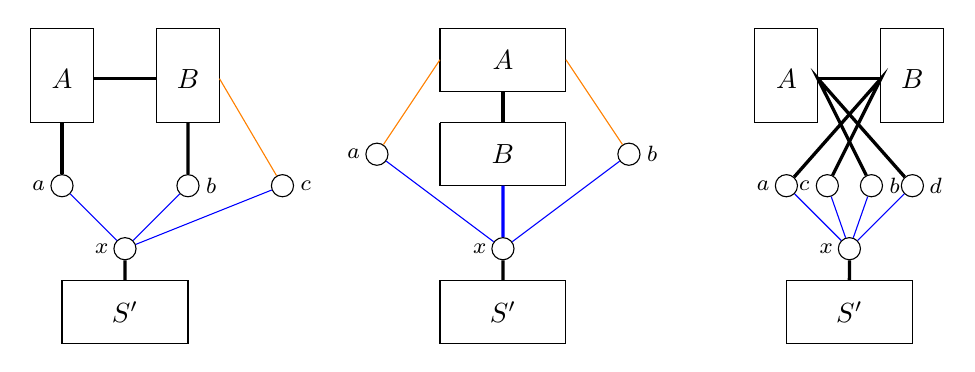
\begin{tikzpicture}[every node/.style={draw,circle,fill=white,inner sep=0pt,minimum size=8pt},every loop/.style={},scale=0.8]

%%%%%% H1
\node[label=left:\footnotesize{$a$}] (a1) at (0,0) {};
\node[label=right:\footnotesize{$b$}] (b1) at (2,0) {};
\node[label=right:\footnotesize{$c$}] (c1) at (3.5,0) {};
\node[label=left:\footnotesize{$x$}] (x1) at (1,-1) {};
\draw (1.5,1)--(2.5,1)--(2.5,2.5)--(1.5,2.5)--(1.5,1);
\draw (-0.5,1)--(0.5,1)--(0.5,2.5)--(-0.5,2.5)--(-0.5,1);
\draw (0,-1.5)--(2,-1.5)--(2,-2.5)--(0,-2.5)--(0,-1.5);
\node[draw=none,fill=none] (A1) at (0,1.7) {$A$};
\node[draw=none,fill=none] (B1) at (2,1.7) {$B$};
\node[draw=none,fill=none] (S1) at (1,-2) {$S'$};

\draw[very thick] (a1)--(0,1);
\draw[very thick] (0.5,1.7)--(1.5,1.7);
\draw[very thick] (b1)--(2,1);
\draw[very thick] (x1)--(1,-1.5);
\draw[color=orange] (c1)--(2.5,1.7);
\draw[color=blue] (x1)--(a1);
\draw[color=blue] (x1)--(b1);
\draw[color=blue] (x1)--(c1);

%%%%%%% H2
\draw (6,2.5)--(8,2.5)--(8,1.5)--(6,1.5)--(6,2.5);
\draw (6,1)--(8,1)--(8,0)--(6,0)--(6,1);
\node[label=left:\footnotesize{$a$}] (a2) at (5,0.5) {};
\node[label=right:\footnotesize{$b$}] (b2) at (9,0.5) {};
\node[label=left:\footnotesize{$x$}] (x2) at (7,-1) {};
\draw (6,-1.5)--(8,-1.5)--(8,-2.5)--(6,-2.5)--(6,-1.5);
\draw[color=orange] (a2)--(6,2);
\draw[color=orange] (b2)--(8,2);
\draw[color=blue] (x2)--(a2);
\draw[color=blue] (x2)--(b2);
\draw[very thick,color=blue] (x2)--(7,0);
\draw[very thick] (x2)--(7,-1.5);
\draw[very thick] (7,1)--(7,1.5);
\node[draw=none,fill=none] (A2) at (7,2) {$A$};
\node[draw=none,fill=none] (B2) at (7,0.5) {$B$};
\node[draw=none,fill=none] (S2) at (7,-2) {$S'$};

%%%%% H3
\draw (11,2.5)--(12,2.5)--(12,1)--(11,1)--(11,2.5);
\draw (13,2.5)--(14,2.5)--(14,1)--(13,1)--(13,2.5);
\node[label=left:\footnotesize{$a$}] (a3) at (11.5,0) {};
\node[label=left:\footnotesize{$c$}] (c3) at (12.15,0) {};
\node[label=right:\footnotesize{$b$}] (b3) at (12.85,0) {};
\node[label=right:\footnotesize{$d$}] (d3) at (13.5,0) {};
\node[label=left:\footnotesize{$x$}] (x3) at (12.5,-1) {};
\draw (11.5,-1.5)--(13.5,-1.5)--(13.5,-2.5)--(11.5,-2.5)--(11.5,-1.5);
\node[draw=none,fill=none] (A3) at (11.5,1.7) {$A$};
\node[draw=none,fill=none] (B3) at (13.5,1.7) {$B$};
\node[draw=none,fill=none] (S3) at (12.5,-2) {$S'$};
\draw[very thick] (x3)--(12.5,-1.5);
\draw[very thick] (12,1.7)--(13,1.7);
\draw[very thick] (a3)--(13,1.7)--(c3);
\draw[very thick] (b3)--(12,1.7)--(d3);
\draw[color=blue] (x3)--(a3);
\draw[color=blue] (x3)--(b3);
\draw[color=blue] (x3)--(c3);
\draw[color=blue] (x3)--(d3);

\end{tikzpicture}
     \caption{The structure of the graphs in the classes, respectively, $\cH_1$, $\cH_2$, and $\cH_3$. Each block denotes an independent set of vertices. A black thick line denotes that there are all possible edges between the sets of vertices, an orange line denotes that there can be some edges between the sets, and a blue line denotes an edge that might (but does not have to) be subdivided.}
    \label{fig:graphs-def}
\end{figure}
\end{center}


\begin{restatable}{lemma}{GirthFourLemmaa}
\label{lem:girth-4-a}
Let $H$ be a graph that is neither a forest nor an induced subgraph of a graph in
$\mathcal H_1\cup \mathcal H_2\cup \mathcal H_3$.
Assume moreover that $\girth(H)\geq 4$.
Then \textsc{$H$-free Subdivision} is NP-hard.
Moreover, assuming the ETH, the problem cannot be solved in time
$2^{o(k)}\cdot n^{O(1)}$.
\end{restatable}

It remains to deal with graphs $H$ that are induced subgraphs of the exceptional classes.
For these graphs the preceding reduction may fail, because an induced copy of $H$ can potentially be distributed across the special dense parts of the construction.
We therefore isolate the possible remaining structures.

Two types of exceptional graphs appear.
The first type is when the vertices that lie on shortest cycles form a robust part of $H$.
More precisely, let $X$ be the set of vertices of $H$ that are contained in at least one shortest cycle.
If $H[X]$ is $2$-connected, then shortest cycles cannot be split across different gadgets that intersect in at most one vertex.
This allows a different version of the Vertex Cover reduction, using a high-girth instance of \textsc{Vertex Cover} as the source problem.

The second type consists of a small number of explicit core structures.
For $k,\ell\geq 2$ and $i_1,i_2,i_3\in\{0,1,2\}$, the graph
$H_{k,\ell}[i_1,i_2,i_3]$ consists of two bundles of internally disjoint $2$-paths, one between $x_1$ and $x_2$ and the other between $x_2$ and $x_3$, together with a vertex $y$ that may be adjacent to, or joined by a subdivided edge to, each of $x_1,x_2,x_3$.
We also need one additional exceptional graph, denoted by $\widetilde H$.

For these exceptional cores, the reduction again starts from a high-girth instance of \textsc{Vertex Cover}.
The use of high girth ensures that short cycles in the constructed graph are confined to individual gadgets.
This allows us to control where the $4$-cycles of a possible induced copy of $H$ can lie.
In the cases where the core is one of the graphs
$H_{k,\ell}[i_1,i_2,i_3]$, the construction sometimes separates $H$ into two parts meeting in a single cut vertex.
One part is attached to an ordered edge of the input graph, and the other part is attached to one endpoint.
This makes every copy of $H$ correspond to an edge of the original graph, while a vertex-cover subdivision again destroys all such copies.


Now let us define the graphs that will be treated separately in \cref{lem:girth-4-b} (see also \cref{fig:special-graph-def}).

Let $k,\ell\geq 2$, and let $i_1,i_2,i_3\in \{0,1,2\}$.
We define the graph $H_{k,\ell}[i_1,i_2,i_3]$ as follows.
Its vertex set is
\[
\{x_1,x_2,x_3,x_{1,1},\ldots,x_{1,k},x_{2,1},\ldots,x_{2,\ell}\}\cup S\cup Y,
\]
where
\[
S:=\{s_j : i_j=2\}\subseteq \{s_1,s_2,s_3\},
\]
and
\[
Y:=
\begin{cases}
\{y\}, & \text{if at least one of } i_1,i_2,i_3 \text{ is non-zero},\\
\emptyset, & \text{otherwise.}
\end{cases}
\]
The edge set is defined as follows:
\begin{enumerate}[(1)]
    \item for every $j\in [k]$, we add the edges $x_1x_{1,j}$ and $x_{1,j}x_2$;
    \item for every $j\in [\ell]$, we add the edges $x_2x_{2,j}$ and $x_{2,j}x_3$;
    \item for every $j\in \{1,2,3\}$:
    \begin{itemize}
        \item if $i_j=0$, then there is no edge between $y$ and $x_j$;
        \item if $i_j=1$, then we add the edge $yx_j$;
        \item if $i_j=2$, then we add the edges $x_js_j$ and $ys_j$, that is, the edge $x_jy$ is subdivided once.
    \end{itemize}
\end{enumerate}

We also define one more special graph, denoted by $\widetilde{H}$, to be the graph on $8$ vertices with
\begin{align*}
    V(\widetilde{H})&=\{x,y,z,t,a_1,a_2,b_1,b_2\}, \\
    E(\widetilde{H})&=\{xa_1,xa_2,a_1y,a_2y,yb_1,yb_2,b_1z,b_2z,tx,tb_2\}.
\end{align*}

\begin{figure}[t]
    \centering
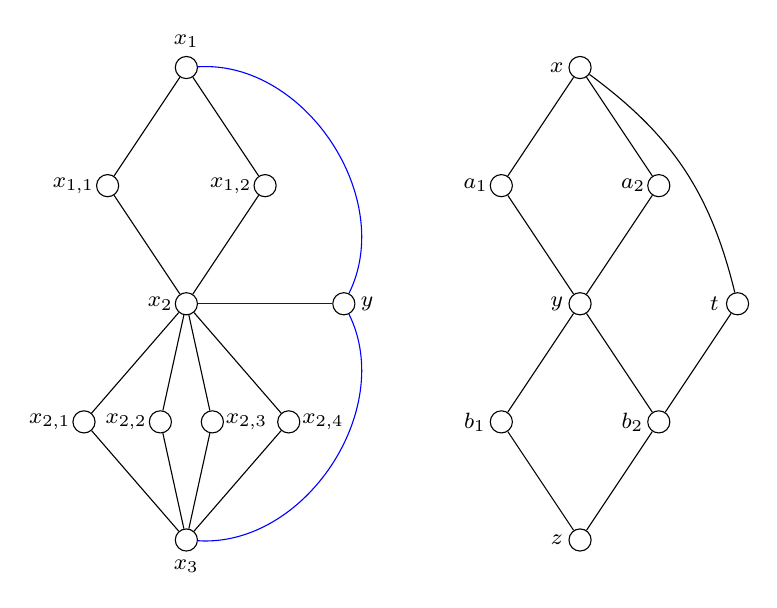
\begin{tikzpicture}[
    every node/.style={draw,circle,fill=white,inner sep=0pt,minimum size=8pt}
]

\node[label=left:\footnotesize{$x_2$}] (a1) at (0,0) {};
\node[label=left:\footnotesize{$x_{2,1}$}] (a2) at (-1.3,-1.5) {};
\node[label=right:\footnotesize{$x_{2,4}$}] (a3) at (1.3,-1.5) {};
\node[label=left:\footnotesize{$x_{1,1}$}] (a4) at (-1,1.5) {};
\node[label=left:\footnotesize{$x_{1,2}$}] (a5) at (1,1.5) {};
\node[label=below:\footnotesize{$x_3$}] (a6) at (0,-3) {};
\node[label=above:\footnotesize{$x_1$}] (a7) at (0,3) {};
\node[label=left:\footnotesize{$x_{2,2}$}] (a8) at (-0.33,-1.5) {};
\node[label=right:\footnotesize{$x_{2,3}$}] (a9) at (0.33,-1.5) {};
\node[label=right:\footnotesize{$y$}] (y) at (2,0) {};

\foreach \k in {2,3,4,5,8,9}{
    \draw (a1)--(a\k);
}

\draw (a6)--(a2);
\draw (a6)--(a3);
\draw (a7)--(a4);
\draw (a7)--(a5);
\draw (a8)--(a6);
\draw (a9)--(a6);

\draw[blue] (a6) to[bend right=60] (y);
\draw[blue] (y) to[bend right=60] (a7);
\draw[blue] (a1)--(y);

%%%%%% \widetilde{H}

\node[label=left:\footnotesize{$y$}] (b1) at (5,0) {};
\node[label=left:\footnotesize{$x$}] (b2) at (5,3) {};
\node[label=left:\footnotesize{$z$}] (b3) at (5,-3) {};
\node[label=left:\footnotesize{$a_1$}] (b4) at (4,1.5) {};
\node[label=left:\footnotesize{$a_2$}] (b5) at (6,1.5) {};
\node[label=left:\footnotesize{$b_1$}] (b6) at (4,-1.5) {};
\node[label=left:\footnotesize{$b_2$}] (b7) at (6,-1.5) {};
\node[label=left:\footnotesize{$t$}] (b8) at (7,0) {};

\draw (b1)--(b4);
\draw (b1)--(b5);
\draw (b1)--(b6);
\draw (b1)--(b7);
\draw (b2)--(b4);
\draw (b2)--(b5);
\draw (b3)--(b6);
\draw (b3)--(b7);
\draw (b2) to[bend left=20] (b8);
\draw (b8)--(b7);

\end{tikzpicture}
\caption{The graph $H_{k,\ell}[i_1,i_2,i_3]$ for $k=2$ and $\ell=4$ (left), and the graph $\widetilde{H}$ (right). The blue line indicates that the corresponding pair of vertices may be non-adjacent, adjacent, or joined by a subdivided edge.}
\label{fig:special-graph-def}
\end{figure}

\begin{restatable}{lemma}{GirthFourLemmab}
\label{lem:girth-4-b}
Let $H$ be a graph that is not a forest and suppose that at least one of the following holds:
\begin{enumerate}[(1)]
    \item the set $X$ of vertices contained in at least one shortest cycle of $H$ induces a $2$-connected subgraph;
    \item $\core(H)$ is isomorphic to $\widetilde{H}$;
    \item there exist $k,\ell\geq 2$ and $i_1,i_2,i_3\in \{0,1,2\}$ such that
    $\core(H)$ is isomorphic to $H_{k,\ell}[i_1,i_2,i_3]$.
\end{enumerate}
Then \textsc{$H$-free Subdivision} is NP-hard.
Moreover, assuming the ETH, the problem cannot be solved in time
$2^{o(k)}\cdot n^{O(1)}$.
\end{restatable}

Let us point out that in \cref{lem:girth-4-b}, there is no assumption on the girth of $H$.
In particular, if $H$ contains precisely one triangle, then the set $X$ of vertices contained in at least one shortest cycle induces a triangle, which clearly is 2-connected.
Therefore, \cref{lem:girth-4-b}~(1) implies \cref{thm:girth3-Unique-Triangle}.

\GirthUniqueTriangle*

The final step is a structural classification.
It shows that the two reductions above, together with the earlier hardness result for graphs whose high-degree vertices induce sufficiently many edges (\cref{thm:easy}), cover all non-forest graphs of girth at least $4$.
Indeed, if $H$ is not covered by the generic reduction of \cref{lem:girth-4-a}, then $H$ must be an induced subgraph of one of the exceptional classes
$\mathcal H_1,\mathcal H_2,\mathcal H_3$.
A case analysis on these three classes shows that either the shortest-cycle vertices induce a $2$-connected graph, or the core of $H$ is one of the explicitly described exceptional cores.

\begin{restatable}{lemma}{GirthFourLemmaAll}
\label{lem:girth-4-all}
Let $H$ be a non-forest induced subgraph of a graph in
$\mathcal H_1\cup \mathcal H_2\cup \mathcal H_3$.
Assume moreover that $H$ does not satisfy the assumptions of \cref{thm:easy}.
Then one of the following holds:
\begin{enumerate}[(1)]
    \item the set $X$ of vertices contained in at least one shortest cycle of $H$ induces a $2$-connected subgraph;\label{it:cycles}
    \item there exist $k,\ell\geq 2$ and $i_1,i_2,i_3\in\{0,1,2\}$ such that
    $\core(H)$ is isomorphic to $H_{k,\ell}[i_1,i_2,i_3]$ or to $\widetilde{H}$.\label{it:special}
\end{enumerate}
\end{restatable}



We can now prove \cref{thm:girth-4}.
Let $H$ be a non-forest graph with $\girth(H)\geq 4$.
If $H$ satisfies the assumptions of \cref{thm:easy}, then the theorem follows from that result.
Otherwise, if $H$ is not an induced subgraph of a graph in
$\mathcal H_1\cup\mathcal H_2\cup\mathcal H_3$, then the theorem follows from
\cref{lem:girth-4-a}.
Finally, if $H$ is an induced subgraph of a graph in
$\mathcal H_1\cup\mathcal H_2\cup\mathcal H_3$, then by \cref{lem:girth-4-all} it satisfies one of the assumptions of \cref{lem:girth-4-b}, and the theorem follows from \cref{lem:girth-4-b}.
The ETH lower bound follows because the reductions used above are parameter-preserving and polynomial-time and from the 
corresponding lower bound of \textsc{Vertex Cover} (\cref{pro:vc}).

\subsection{Formal proofs}
We now give the formal proofs.
%\begin{theorem}\label{thm:girth-4}
%Let $H$ be a graph which is not a forest and such that $\girth(H)\geq 4$.
%Then \textsc{$H$-free Subdivision} is NP-complete. Further, assuming the ETH, the problem cannot be solved in time
%$2^{o(k)}\cdot n^{O(1)}$.
%\end{theorem}

%We split the proof of \cref{thm:girth-4} into two cases, depending on the properties of the graph $H$.
%We perform two reductions in \cref{lem:girth-4-a} and \cref{lem:girth-4-b}, and then in \cref{lem:girth-4-all} we show that every graph $H$ that satisfies the assumptions of \cref{thm:girth-4} satisfies also the assumptions either of \cref{lem:girth-4-a} or \cref{lem:girth-4-b}.


% In the definition of \cH_1, replace item (4) by:


% In the definition of \cH_2, replace item (4) by:

\GirthFourLemmaa*

\begin{proof}
We may assume that $H$ does not satisfy the assumptions of
Theorem~\ref{thm:easy}.
Let $X\subseteq V(H)$ be the set of vertices of degree at least $3$.
Then $H[X]$ contains at most one edge.

Since $H$ is not a forest, it contains a cycle.
Let $C=c_1c_2\ldots c_\ell c_1$ be a shortest cycle in $H$, where
$\ell=\girth(H)\geq 4$.
We claim that some vertex of $C$ has degree exactly $2$ in $H$.
Indeed, if every vertex of $C$ had degree at least $3$, then every edge of $C$
would lie in $H[X]$, and hence $H[X]$ would contain at least $\ell\geq 4$ edges,
contrary to our assumption on $H[X]$.
Fix such a vertex and denote it by $c$.
Let $a$ and $b$ be the two neighbors of $c$ in $H$.

We reduce from \textsc{Vertex Cover}.
Let $(G,k)$ be an instance of \textsc{Vertex Cover}.
We construct an instance $(G',k)$ of \textsc{$H$-free Subdivision} as follows.

Start with an independent set $V(G)$.
Add one new vertex $z$ and make it adjacent to every vertex of $V(G)$.
For every edge $e=uv\in E(G)$, introduce a set $X_e$ of fresh vertices and add
edges so that the graph induced by
\[
X_e\cup \{u,v,z\}
\]
is isomorphic to $H$, where $z$ corresponds to $c$ and $u,v$ correspond to the
two neighbors $a,b$ of $c$.
Since $c$ has degree exactly $2$ in $H$, no further edges incident with $z$
inside this copy are needed.

Finally, for every two distinct edges $e,f\in E(G)$, add all edges between
$X_e$ and $X_f$, and for every $w\in V(G)$ and every edge $e=uv\in E(G)$ with
$w\notin \{u,v\}$, add all edges between $w$ and $X_e$.

This finishes the construction of $G'$.
It is clearly polynomial-time computable.

We now prove correctness.

\smallskip
\noindent
\emph{If $(G',k)$ is a yes-instance, then $(G,k)$ is a yes-instance of
\textsc{Vertex Cover}.}
Suppose that by at most $k$ subdivisions of $G'$ we obtain an $H$-free graph
$G^\star$.
We build a set $Y\subseteq V(G)$ as follows.

For every $v\in V(G)$, if the edge $zv$ was subdivided, then put $v$ into $Y$.
Further, for every edge $e=uv\in E(G)$, if some subdivided edge lies in the graph
induced by $X_e\cup\{u,v,z\}$ and is different from $zu$ and $zv$, then put
one arbitrarily chosen endpoint of $e$ into $Y$.

Clearly, $|Y|\leq k$.

We claim that $Y$ is a vertex cover of $G$.
Fix an edge $e=uv\in E(G)$.
By construction, $G'[X_e\cup\{u,v,z\}]$ is an induced copy of $H$.
Subdividing an edge outside this vertex set does not change the induced subgraph
on this set.
Hence, in order to destroy this copy of $H$, at least one subdivided edge must lie
inside $X_e\cup\{u,v,z\}$.
If the subdivided edge is $zu$ or $zv$, then $u\in Y$ or $v\in Y$ by construction.
Otherwise, we added one of $u,v$ to $Y$ when processing the edge $e$.
Thus $Y\cap\{u,v\}\neq\emptyset$.
Since this holds for every edge $uv\in E(G)$, the set $Y$ is a vertex cover of $G$.

\smallskip
\noindent
\emph{If $(G,k)$ is a yes-instance of \textsc{Vertex Cover}, then $(G',k)$ is a
yes-instance of \textsc{$H$-free Subdivision}.}
Let $Y\subseteq V(G)$ be a vertex cover of $G$ of size at most $k$.
Construct $G^\star$ from $G'$ by subdividing, for every $v\in Y$, the edge $zv$.
Let $S$ be the set of new subdivision vertices.
We performed at most $k$ subdivisions.

Assume for a contradiction that $G^\star$ contains an induced subgraph $F$
isomorphic to $H$.
Since $\girth(H)\geq 4$, the graph $H$ is triangle-free, and hence so is $F$.

For an edge $e\in E(G)$, let
\[
X_e^F:=X_e\cap V(F).
\]
The graph induced by $V(G)\cup S\cup\{z\}$ is a subdivided star and therefore
acyclic.
Since $H$ is not a forest, the copy $F$ must contain a vertex of $X_e$ for some
$e\in E(G)$.
Thus $X_e^F\neq\emptyset$ for some $e$.

We first show that there are vertices of $F$ in at most two distinct sets
$X_e$.
Indeed, if $X_e^F$, $X_f^F$, and $X_g^F$ were all nonempty for three distinct edges
$e,f,g\in E(G)$, then choosing one vertex from each set would give a triangle in
$F$, because all edges between distinct $X$-sets are present in $G'$.
This is impossible.
Hence there are at most two edges of $G$ whose $X$-sets meet $V(F)$.

We now distinguish cases.

\subparagraph*{Case 1: \boldmath $X_{uv}^F\neq\emptyset$ and $X_{vw}^F\neq\emptyset$ for two edges
sharing an endpoint.}
Then $u,v,w$ are distinct.
Every vertex of $V(G)\setminus\{u,v,w\}$ is adjacent to all vertices of
$X_{uv}\cup X_{vw}$ by construction.
Therefore such a vertex cannot belong to $F$, for otherwise together with one
vertex of $X_{uv}^F$ and one vertex of $X_{vw}^F$ it would form a triangle.
Hence
\[
V(F)\subseteq \{u,v,w,z\}\cup S\cup X_{uv}\cup X_{vw}.
\]

Moreover, each of $X_{uv}^F$ and $X_{vw}^F$ is an independent set, for otherwise
an edge inside one of them together with a vertex from the other nonempty set would
again yield a triangle.

Next, if $u\in V(F)$, then $u$ is anticomplete to $X_{uv}^F$.
Indeed, if $u$ had a neighbor in $X_{uv}^F$, then, since $u\notin\{v,w\}$,
the vertex $u$ is adjacent to every vertex of $X_{vw}^F$, and we obtain a triangle.
Similarly, if $w\in V(F)$, then $w$ is anticomplete to $X_{vw}^F$.
Also, if $v\in V(F)$, then $v$ can be adjacent to vertices of at most one of the
sets $X_{uv}^F$ and $X_{vw}^F$; otherwise we again obtain a triangle.

Now set
\[
A:=X_{vw}^F,\qquad B:=X_{uv}^F,
\]
let $x$ correspond to $z$, let $a$ correspond to $u$ if $u\in V(F)$, let $b$
correspond to $w$ if $w\in V(F)$, and let $c$ correspond to $v$ if $v\in V(F)$.
Put into $S$ the vertices of $F$ lying on subdivided edges among
$\{zu,zv,zw\}$, and put all remaining subdivision vertices of $F$ into $S'$.

The observations above imply that $F$ is an induced subgraph of a graph in $\cH_1$,
contrary to the assumption of the lemma.

\subparagraph*{Case 2: \boldmath $X_{uv}^F\neq\emptyset$ and $X_{wq}^F\neq\emptyset$ for two
vertex-disjoint edges.}
As above, every vertex of $V(G)\setminus\{u,v,w,q\}$ is adjacent to all vertices of
$X_{uv}\cup X_{wq}$, and therefore cannot belong to $F$.
Thus
\[
V(F)\subseteq \{u,v,w,q,z\}\cup S\cup X_{uv}\cup X_{wq}.
\]

Again, $X_{uv}^F$ and $X_{wq}^F$ are independent sets.
Also, if $u\in V(F)$ or $v\in V(F)$, then that vertex is anticomplete to $X_{uv}^F$,
since it is complete to $X_{wq}^F$.
Similarly, if $w\in V(F)$ or $q\in V(F)$, then that vertex is anticomplete to
$X_{wq}^F$.

Now set
\[
A:=X_{uv}^F,\qquad B:=X_{wq}^F,
\]
let $x$ correspond to $z$, and let $a,c,b,d$ correspond to
$u,v,w,q$, respectively, whenever these vertices belong to $F$.
Put into $S$ the subdivision vertices of $F$ lying on the subdivided edges among
$\{zu,zv,zw,zq\}$, and put all remaining subdivision vertices of $F$ into $S'$.

Then $F$ is an induced subgraph of a graph in $\cH_3$, again a contradiction.

\subparagraph*{Case 3: exactly one set \boldmath $X_{uv}$ meets $V(F)$.}
So $X_{uv}^F\neq\emptyset$ and $X_e^F=\emptyset$ for every other edge $e\in E(G)$.

First suppose that $F$ contains a vertex $y\in V(G)\setminus\{u,v\}$.
Since $y$ is complete to $X_{uv}$, the set $X_{uv}^F$ must be independent.
Now set
\[
A:=X_{uv}^F,\qquad B:=V(F)\cap (V(G)\setminus\{u,v\}),
\]
let $x$ correspond to $z$, and let $a,b$ correspond to $u,v$, respectively,
whenever they belong to $F$.
Put into $S$ the subdivision vertices of $F$ lying on subdivided edges $zy$ with
$y\in V(F)\cap V(G)$, and put all remaining subdivision vertices of $F$ into $S'$.
Then $F$ is an induced subgraph of a graph in $\cH_2$, a contradiction.

Thus no vertex of $V(G)\setminus\{u,v\}$ belongs to $F$.
Therefore
\[
V(F)\subseteq \{u,v,z\}\cup S\cup X_{uv}.
\]

Since $Y$ is a vertex cover of $G$ and $uv\in E(G)$, at least one of $u$ and $v$
belongs to $Y$.
Hence at least one of the two edges $zu$ and $zv$ was subdivided when passing from
$G'$ to $G^\star$.

Consider the graph
\[
Q:=G^\star[\{u,v,z\}\cup X_{uv}\cup S].
\]
%Vertices of $S$ that do not lie on a subdivided edge incident with $u$ or $v$
%have degree at most one in $Q$, and therefore lie on no cycle of $Q$.
The graph $G'[\{u,v,z\}\cup X_{uv}]$ is isomorphic to $H$, and in this copy the
vertex corresponding to $c$ is $z$.
In particular, $Q$ contains all cycles of that copy of $H$ except that every cycle
using a subdivided edge $zu$ or $zv$ has its length increased by one.
Hence subdividing $zu$ and/or $zv$ destroys at least one cycle of length $\ell$,
namely a shortest cycle containing $z$, and it creates no new cycle of length $\ell$.

Consequently, the total number of $\ell$-cycles in $Q$ is strictly smaller than the
number of $\ell$-cycles in $H$.
Therefore $Q$ cannot contain an induced copy of $H$.
Since $F$ is an induced subgraph of $Q$ and isomorphic to $H$, this is impossible.

All cases lead to a contradiction.
Hence $G^\star$ is $H$-free, and $(G',k)$ is a yes-instance of
\textsc{$H$-free Subdivision}.
%This completes the proof.
Now the statements follow from \cref{pro:vc}.
\end{proof}

Now we are ready to prove the following.

\GirthFourLemmab*

\begin{proof}
We may assume that $H$ does not satisfy the assumptions of \cref{thm:easy}.
We reduce from \textsc{Vertex Cover}.
Let $(G,p)$ be an instance of \textsc{Vertex Cover} such that $\girth(G)>|V(H)|$.
We construct an equivalent instance $(G',p)$ of \textsc{$H$-free Subdivision}.
The construction depends on which of the above conditions is satisfied by $H$.

\subparagraph*{Case 1: \boldmath $H$ satisfies~(1), or $\core(H)\cong \widetilde{H}$, or $\core(H)\cong H_{k,\ell}[i_1,i_2,i_3]$ with $i_1,i_3\neq 0$.}
We first choose a special vertex $\tc$ of degree exactly $2$ in $H$.

Assume first that $H$ satisfies~(1).
Let $c_1,\ldots,c_r$ be consecutive vertices of a shortest cycle in $H$.
Since $H$ is not a forest, such a cycle exists.
Observe that some vertex $c_i$ on this cycle has degree exactly $2$.
Indeed, otherwise every vertex of this shortest cycle would have degree at least $3$, and then $H$ would satisfy the assumptions of \cref{thm:easy}, a contradiction.
We set $\tc:=c_i$.

If $\core(H)\cong \widetilde{H}$, then we set $\tc$ to be the vertex corresponding to $a_1$.
Its degree in $H$ is at least its degree in $\core(H)$, and hence at least $2$.
On the other hand, its degree in $H$ cannot exceed $2$, for otherwise $H$ would satisfy the assumptions of \cref{thm:easy}.

Finally, suppose that $\core(H)\cong H_{k,\ell}[i_1,i_2,i_3]$ with $i_1,i_3\neq 0$.
By symmetry, we may assume that $k\leq \ell$.
We set $\tc:=x_{1,1}$.
Again, $x_{1,1}$ has degree exactly $2$ in $H$; otherwise $H$ would satisfy the assumptions of \cref{thm:easy}.

Let $a$ and $b$ be the two neighbors of $\tc$ in $H$.

We now construct $(G',p)$.
Start with the graph with vertex set $V(G)\cup \{q\}$ and edge set
\[
\{qv : v\in V(G)\};
\]
in particular, $V(G)$ is an independent set in $G'$.
For every edge $uv\in E(G)$, introduce a set $X_{uv}$ of fresh vertices and add edges inside
\[
X_{uv}\cup \{u,v\}
\]
so that the induced subgraph
\[
G'[X_{uv}\cup \{u,v,q\}]
\]
is isomorphic to $H$, with $q$ corresponding to $\tc$ and $u,v$ corresponding to $a,b$, respectively.
Observe that we do not add any new edge incident with $q$; all additional edges are added inside $X_{uv}\cup \{u,v\}$.
This completes the construction in Case~1.

\subparagraph*{Case 2: \boldmath $\core(H)\cong H_{k,\ell}[i_1,i_2,i_3]$ and at most one of $i_1,i_3$ is non-zero.}
By symmetry, we may assume that $i_3=0$.
Moreover, if $i_1\neq 0$, then necessarily $i_2\neq 0$, since otherwise the vertex $y$ would have degree $1$ in $\core(H)$, impossible.
We may also assume that it is not the case that $i_1=i_2=1$, because then $\core(H)\cong H_{k+1,\ell}[0,0,0]$.

Fix an isomorphism from $\core(H)$ to $H_{k,\ell}[i_1,i_2,i_3]$.
Let $L$ and $R$ be the vertex sets of the two connected components of $\core(H)-x_2$, where $L$ is the component containing $x_1$ and $R$ is the component containing $x_3$.
Thus $\core(H)-x_2$ has exactly two components.

We define two vertex sets $V_1,V_2\subseteq V(H)$ as follows.
First put $x_2$ in both $V_1$ and $V_2$.
For every connected component $C$ of $H-x_2$,
\begin{itemize}
    \item if $C$ contains a vertex of $L$, then put $V(C)$ into $V_1$;
    \item if $C$ contains a vertex of $R$, then put $V(C)$ into $V_2$;
    \item if $C$ is disjoint from $\core(H)$, then put $V(C)$ into $V_1$.
\end{itemize}
Since every vertex of $H\setminus \core(H)$ lies in a tree attached to a unique vertex of $\core(H)$, this definition is unambiguous.
Moreover,
\[
V_1\cup V_2=V(H), \qquad V_1\cap V_2=\{x_2\},
\]
and there are no edges between $V_1\setminus \{x_2\}$ and $V_2\setminus \{x_2\}$.

Furthermore, at least one of $x_{1,1},\ldots,x_{1,k}$ has degree exactly $2$ in $H$.
Indeed, otherwise at least two of these vertices would have degree at least $3$, and together with $x_2$ they would force the assumptions of \cref{thm:easy}.
By symmetry, we may assume that $x_{1,1}$ has degree exactly $2$.
Similarly, we may assume that $x_{2,1}$ has degree exactly $2$.

Now we perform the construction.
Start with the graph with vertex set $V(G)\cup \{q\}$ and edge set
\[
\{qv : v\in V(G)\};
\]
again, $V(G)$ is an independent set.

\subparagraph*{Subcase 2.1: \boldmath $k\leq \ell$.}
For every ordered pair $(u,v)$ such that $uv\in E(G)$, introduce a set $X_{uv}$ of fresh vertices and add edges so that
\[
G'[X_{uv}\cup \{u,v,q\}]
\]
is isomorphic to $H[V_1]$, with $q$ corresponding to $x_{1,1}$, $u$ corresponding to $x_1$, and $v$ corresponding to $x_2$.
Furthermore, for every $v\in V(G)$, introduce a set $X_v$ of fresh vertices and add edges so that
\[
G'[X_v\cup \{v\}]
\]
is isomorphic to $H[V_2]$, with $v$ corresponding to $x_2$.
Thus, for every ordered pair $(u,v)$ with $uv\in E(G)$, the graph
\[
G'[X_{uv}\cup X_v\cup \{u,v,q\}]
\]
is isomorphic to $H$.

\subparagraph*{Subcase 2.2: \boldmath $k>\ell$.}
For every ordered pair $(u,v)$ such that $uv\in E(G)$, introduce a set $X_{uv}$ of fresh vertices and add edges so that
\[
G'[X_{uv}\cup \{u,v,q\}]
\]
is isomorphic to $H[V_2]$, with $q$ corresponding to $x_{2,1}$, $u$ corresponding to $x_3$, and $v$ corresponding to $x_2$.
Furthermore, for every $v\in V(G)$, introduce a set $X_v$ of fresh vertices and add edges so that
\[
G'[X_v\cup \{v\}]
\]
is isomorphic to $H[V_1]$, with $v$ corresponding to $x_2$.
Thus, for every ordered pair $(u,v)$ with $uv\in E(G)$, the graph
\[
G'[X_{uv}\cup X_v\cup \{u,v,q\}]
\]
is isomorphic to $H$.

\subparagraph*{Correctness.}
Assume first that $(G',p)$ is a yes-instance of \textsc{$H$-free Subdivision}, and let $G''$ be obtained from $G'$ by at most $p$ edge subdivisions so that $G''$ is $H$-free.
We define a set $Y\subseteq V(G)$ as follows.
We add to $Y$ every vertex $v$ such that the edge $vq$ was subdivided.
Moreover, for every ordered pair $(u,v)$ with $uv\in E(G)$, if at least one edge inside $X_{uv}\cup \{u,v\}$ was subdivided, then we arbitrarily add one of $u,v$ to $Y$.
Finally, if $G'$ was constructed in Case~2 and at least one edge inside $X_v$ was subdivided, then we add $v$ to $Y$.
Clearly, $|Y|\leq p$.

We claim that $Y$ is a vertex cover of $G$.
Consider an edge $uv\in E(G)$.
If $G'$ was constructed in Case~1, then $X_{uv}\cup \{u,v,q\}$ induces a copy of $H$ in $G'$.
Hence at least one edge of this induced subgraph must be subdivided, and therefore at least one of $u,v$ was added to $Y$.
If $G'$ was constructed in Case~2, then the graph
\[
G'[X_{uv}\cup X_v\cup \{u,v,q\}]
\]
is isomorphic to $H$.
Again, at least one edge of this induced subgraph must be subdivided, and therefore at least one of $u,v$ was added to $Y$.
Thus $Y$ is a vertex cover of $G$.

Now suppose that $(G,p)$ is a yes-instance of \textsc{Vertex Cover}, and let $Y$ be a vertex cover of $G$ of size at most $p$.
We obtain $G''$ from $G'$ by subdividing the edge $vq$ for every $v\in Y$.
Clearly, we perform at most $p$ subdivisions.
We show that $G''$ is $H$-free.

Assume for a contradiction that $G''$ contains an induced copy $F$ of $H$.
We distinguish the following cases.

\subparagraph*{Case 1: the set of vertices contained in a shortest cycle of \boldmath $H$ induces a $2$-connected subgraph.}
Let $g:=\girth(H)$.
We first show that the vertex $q$ is not contained in any $g$-cycle of $G''$.
Suppose otherwise that $C$ is a $g$-cycle containing $q$, and let $u,v\in V(G)$ be the neighbors of $q$ on $C$.
Every $u$--$v$ path in $G''-q$ traverses, for each edge of the corresponding walk in $G$, a gadget in which the distance between the corresponding branch vertices is at least $g-2$.
Hence
\[
\dist_{G''-q}(u,v)\geq (g-2)\cdot \dist_G(u,v).
\]
If $uv\notin E(G)$, then $\dist_G(u,v)\geq 2$, and thus
\[
|C|\geq 2+2(g-2)=2g-2>g,
\]
a contradiction.
Hence $uv\in E(G)$.
But then, since $Y$ is a vertex cover of $G$, at least one of $u$ and $v$ belongs to $Y$, and therefore at least one of the edges $uq,vq$ was subdivided in $G''$.
Consequently,
\[
|C|\geq 3+(g-2)=g+1,
\]
again a contradiction.

Thus every $g$-cycle of $F$ avoids $q$.
Since $\girth(G)>|V(H)|\geq g$, every $g$-cycle of $G''$ is contained in $X_{uv}\cup \{u,v\}$ for some edge $uv\in E(G)$.
Let $X$ be the set of vertices of $H$ contained in at least one shortest cycle.
By assumption, $H[X]$ is $2$-connected.
Therefore the corresponding vertex set in $F$ is contained in a single set $X_{uv}\cup \{u,v\}$, since two distinct such sets intersect in at most one vertex.
Now $G'[X_{uv}\cup \{u,v,q\}]$ is a copy of $H$ in which $q$ lies on a shortest cycle, whereas in $G''[X_{uv}\cup \{u,v\}]$ all shortest cycles through the vertex corresponding to $q$ have been destroyed.
Hence the number of $g$-cycles in $G''[X_{uv}\cup \{u,v\}]$ is strictly smaller than in $H$, a contradiction.

\subparagraph*{Case 2: \boldmath $\core(H)\cong \widetilde{H}$.}
For every edge $uv\in E(G)$, the set $X_{uv}\cup \{u,v,q\}$ induces a copy of $H$ with $q$ corresponding to $a_1$.
As in Case~1, the vertex $q$ is not contained in any $4$-cycle of $G''$.
Indeed, $q$ is adjacent only to vertices of $V(G)$, and if $u,v\in V(G)$ then any cycle through $q,u,v$ has length at least $5$: if $uv\notin E(G)$, then every $u$--$v$ path avoiding $q$ has length at least $4$; and if $uv\in E(G)$, then at least one of the edges $uq,vq$ was subdivided.

Since $\girth(G)>|V(H)|\geq 8$, every $4$-cycle in $G''$ is contained in $X_{uv}\cup \{u,v\}$ for some edge $uv\in E(G)$.
In each such set there is precisely one $4$-cycle.
Hence, in an induced copy of $\widetilde{H}$ in $G''$, the two $4$-cycles of $\widetilde{H}$ must be realized in two gadgets sharing a vertex of $V(G)$.
Thus there exist $u,v,w\in V(G)$ with $uv,vw\in E(G)$ such that
\[
a_1,a_2\in X_{uv},\qquad x\in X_{uv}\cup \{u\},\qquad y=v,\qquad
b_1,b_2\in X_{vw},\qquad z\in X_{vw}\cup \{w\}.
\]
Now the vertex corresponding to $t$ must be adjacent to $b_2$, so it lies in $X_{vw}\cup \{w\}$, since it is different from $y=v$.
On the other hand, it must also be adjacent to $x\in X_{uv}\cup \{u\}$.
No such vertex exists in $G''$, a contradiction.

\subparagraph*{Case 3: \boldmath $\core(H)\cong H_{k,\ell}[i_1,i_2,i_3]$ with $i_1,i_3>0$.}
In this case, for every edge $uv\in E(G)$, the set $X_{uv}\cup \{u,v,q\}$ induces a graph isomorphic to $H$ with $q$ corresponding to $x_{1,1}$.
As in the previous cases, the vertex $q$ is not contained in any $4$-cycle of $G''$.
Furthermore, since $\girth(G)>|V(H)|>4$, every $4$-cycle of $G''$ is fully contained in $X_{uv}\cup \{u,v\}$ for some $uv\in E(G)$.

Applying this observation to the two sides of the core, we obtain that, for any induced copy of $H$ in $G''$, all vertices of
\[
\{x_1,x_{1,1},\ldots,x_{1,k},x_2\}
\]
must be contained in one such set $X_{uv}\cup \{u,v\}$, and all vertices of
\[
\{x_2,x_{2,1},\ldots,x_{2,\ell},x_3\}
\]
must be contained in one such set $X_{vw}\cup \{v,w\}$.

Suppose first that these two sets coincide.
Then
\[
\{x_1,x_{1,1},\ldots,x_{1,k},x_2,x_{2,1},\ldots,x_{2,\ell},x_3\}\subseteq X_{uv}\cup \{u,v\}.
\]
If $i_1=i_2=1$ or $i_2=i_3=1$, then also $y\in X_{uv}\cup \{u,v\}$, since it is adjacent to at least two vertices of this set.
If this is not the case, then $y$ is not contained in any $4$-cycle of $H$.
Thus every vertex of $H$ that lies on a $4$-cycle is contained in $X_{uv}\cup \{u,v\}$.
But the graph induced by $X_{uv}\cup \{u,v\}$ contains strictly fewer $4$-cycles than $H$, because the $4$-cycles through the vertex corresponding to $q$ were destroyed when we subdivided at least one edge incident with $q$.
This is a contradiction.

Hence there exist $u,v,w\in V(G)$ with $uv,vw\in E(G)$ such that
\[
x_2=v,
\]
\[
x_1,x_{1,1},\ldots,x_{1,k}\in X_{uv}\cup \{u\},
\]
and
\[
x_{2,1},\ldots,x_{2,\ell},x_3\in X_{vw}\cup \{w\}.
\]

Suppose first that $x_1=u$.
Then the vertices $x_{1,1},\ldots,x_{1,k}$ must all be adjacent to both $u=x_1$ and $v=x_2$.
Recall that $q$ corresponds to $x_{1,1}$, and at least one of the edges $uq$ and $vq$ was subdivided in $G''$.
Hence $q$ is adjacent to at most one of $u$ and $v$, and so $q$ cannot play the role of any of the vertices $x_{1,1},\ldots,x_{1,k}$ in the induced copy.

Therefore, inside $G''[X_{uv}\cup \{u,v,q\}]$, the only vertices adjacent to both $u$ and $v$ are the $k-1$ vertices corresponding to $x_{1,2},\ldots,x_{1,k}$, and, additionally, the vertex corresponding to $y$ if and only if $i_1=i_2=1$.
Consequently, $x_1=u$ is possible only if $i_1=i_2=1$.

Assume now that $i_1=i_2=1$.
Then the $k$ common neighbors of $u$ and $v$ in $G''[X_{uv}\cup \{u,v,q\}]$ are exactly the vertices that must realize $x_{1,1},\ldots,x_{1,k}$.
However, the vertex $y$ is distinct from all of $x_{1,1},\ldots,x_{1,k}$ and is also adjacent to both $x_1$ and $x_2$.
Thus $y$ would require one more common neighbor of $u$ and $v$, but no such vertex exists.
This contradiction shows that $x_1\neq u$.

Hence $x_1\in X_{uv}$.
Since $i_1>0$, the distance between $x_1$ and $y$ in $H$ is at most $2$.
As $x_2=v$, every vertex of $G''$ at distance at most $2$ from $x_1$ and different from $v$ lies in $X_{uv}\cup \{u\}$.
Therefore,
\[
y\in X_{uv}\cup \{u\}.
\]

Now suppose that $x_3=w$.
Since $i_3>0$, the distance between $x_3$ and $y$ in $H$ is at most $2$.
As $x_2=v$, every vertex of $G''$ at distance at most $2$ from $x_3$ and different from $v$ lies in $X_{vw}\cup \{w\}$.
Therefore,
\[
y\in X_{vw}\cup \{w\}.
\]
Since the sets $X_{uv}\cup \{u\}$ and $X_{vw}\cup \{w\}$ are disjoint, this is impossible.
Hence $x_3\neq w$, and therefore $x_3\in X_{vw}$.

Now $y$ must be at distance at most $2$ from both $x_1$ and $x_3$.
Consequently,
\[
y\in X_{uv}\cup \{u\}
\qquad\text{and}\qquad
y\in X_{vw}\cup \{w\},
\]
again a contradiction.

\subparagraph*{Case 4: \boldmath $\core(H)\cong H_{k,\ell}[i_1,i_2,i_3]$ with $i_1=0$ or $i_3=0$.}
As in the previous cases, the vertex $q$ is not contained in any $4$-cycle of $G''$.
Moreover, every $4$-cycle of $G''$ is either fully contained in $X_{uv}\cup \{u,v\}$ for some ordered pair $(u,v)$ with $uv\in E(G)$, or fully contained in $X_v\cup \{v\}$ for some $v\in V(G)$.
Therefore, for an induced copy of $H$, the vertices
\[
\{x_1,x_{1,1},\ldots,x_{1,k},x_2\}
\]
must be fully contained either in $X_{uv}\cup \{u,v\}$ for some ordered pair $(u,v)$ with $uv\in E(G)$, or in $X_v\cup \{v\}$ for some $v\in V(G)$.
Similarly, the vertices
\[
\{x_2,x_{2,1},\ldots,x_{2,\ell},x_3\}
\]
must be fully contained either in $X_{vw}\cup \{v,w\}$ for some ordered pair $(v,w)$ with $vw\in E(G)$, or in $X_v\cup \{v\}$ for some $v\in V(G)$.

By the construction of $G'$ in this case, there must exist $u,v,w\in V(G)$ with $uv,vw\in E(G)$ such that $x_2=v$ and the set
\[
\{x_1,x_{1,1},\ldots,x_{1,k}\}
\]
is contained either in $X_{uv}\cup \{u\}$ or in $X_v$, and the set
\[
\{x_{2,1},\ldots,x_{2,\ell},x_3\}
\]
is contained either in $X_{vw}\cup \{w\}$ or in $X_v$.
Recall that we assumed that it is not the case that $i_1=i_2=1$.

Suppose first that $k\leq \ell$.
Then there are only $k-1$ vertices in $X_{uv}$ adjacent to both $u$ and $v$, and only $\ell-1$ vertices in $X_{vw}$ adjacent to both $v$ and $w$.
Hence neither
\[
\{x_1,x_{1,1},\ldots,x_{1,k}\}
\]
nor
\[
\{x_{2,1},\ldots,x_{2,\ell},x_3\}
\]
can be realized inside $X_{uv}\cup \{u\}$ or $X_{vw}\cup \{w\}$, respectively.
Therefore both sets must be contained in $X_v$.
But then $X_v$ contains only $\ell+1$ vertices that lie on a $4$-cycle, while
\[
\{x_1,x_{1,1},\ldots,x_{1,k}\}\cup \{x_{2,1},\ldots,x_{2,\ell},x_3\}
\]
contains
\[
(k+1)+(\ell+1)-1 = k+\ell+1 \geq \ell+3
\]
such vertices, a contradiction.

Finally, suppose that $\ell<k$.
By the symmetric argument, both sets must again be contained in $X_v$.
However, now $X_v$ contains only $k+1$ vertices that lie on a $4$-cycle, while the same union contains at least
\[
k+\ell+1 \geq k+3
\]
such vertices, again a contradiction.

In all cases we obtain a contradiction.
%Hence $G''$ is $H$-free, and therefore \textsc{$H$-free Subdivision} is NP-hard.
Now the statements follow from \cref{pro:vc}.
\end{proof}

Now we show that the above reductions, together with \cref{thm:easy}, cover all non-forests of girth at least four.

\GirthFourLemmaAll*

\begin{proof}
We consider the cases depending on $i\in [3]$ such that $H$ is an induced subgraph of a graph in $\cH_i$.

\subparagraph*{Case 1: \boldmath $H$ is an induced subgraph of a graph in $\cH_1$.}
Since $H$ does not satisfy the assumptions of \cref{thm:easy}, we cannot have both $|A|\geq 3$ and $|B|\geq 3$, because then all vertices of $A\cup B$ would have degree at least $3$ and all edges between $A$ and $B$ would be present.
We also cannot have $B=\emptyset$, as then $H$ is a forest.

\subparagraph*{Subcase 1.1: \boldmath $|A|,|B|\geq 2$.}
Then $\girth(H)=4$, and each vertex of $A\cup B$ lies on some $4$-cycle.
Moreover, the $4$-cycles in $H$ are of the following types:
\begin{itemize}
    \item $4$-cycles contained in $A\cup B$;
    \item cycles containing $a$, two vertices of $A$, and one vertex of $B$;
    \item cycles containing $b$, two vertices of $B$, and one vertex of $A$;
    \item cycles containing $x,b,c$, and one vertex of $B$ (in this case $c$ must be adjacent to at least one vertex of $B$);
    \item cycles containing $c$, two vertices of $B$, and one vertex of $A$ (in this case $c$ must be adjacent to at least two vertices of $B$).
\end{itemize}
Therefore, $H$ satisfies~\ref{it:cycles}.

\subparagraph*{Subcase 1.2: \boldmath $|A|=1$, $|B|\geq 2$.}
If $b\in V(H)$, then $\girth(H)=4$.
The $4$-cycles in $H$ are:
\begin{itemize}
    \item cycles containing the vertex of $A$, two vertices of $B$, and $b$;
    \item cycles containing the vertex of $A$, two vertices of $B$, and $c$ (in this case $c$ must be adjacent to at least two vertices of $B$);
    \item cycles containing $x,b,c$, and one vertex of $B$ (in this case $c$ must be adjacent to at least one vertex of $B$).
\end{itemize}
Hence $H$ satisfies~\ref{it:cycles}.

If $b\notin V(H)$, then $c\in V(H)$ and $c$ must be adjacent to at least one vertex of $B$, otherwise $H$ would be a forest.
If, in addition, $c$ is adjacent to at least two vertices of $B$, then $\girth(H)=4$, and every $4$-cycle of $H$ consists of the vertex of $A$, two vertices of $B$, and $c$.
Thus again $H$ satisfies~\ref{it:cycles}.
If $c$ is adjacent to at most one vertex of $B$, then every cycle in $H$ contains $a$, the unique vertex of $A$, one vertex of $B$, $c$, and $x$, so $H$ satisfies~\ref{it:cycles}.

\subparagraph*{Subcase 1.3: \boldmath $A=\emptyset$.}
Since $H$ is not a forest, we have $b,c\in V(H)$ and $c$ is adjacent to at least one vertex of $B$.
If $|B|\geq 2$ and $c$ is adjacent to at least two vertices of $B$, then $\girth(H)=4$.
Every $4$-cycle in $H$ must contain $b,c$ and either two vertices of $B$ or one vertex of $B$ together with $x$, and thus $H$ satisfies~\ref{it:cycles}.
If $c$ is adjacent to at most one vertex of $B$, then there is only one cycle in $H$, and this cycle contains $b,x,c$, and the unique neighbor of $c$ in $B$.
Hence again $H$ satisfies~\ref{it:cycles}.

\subparagraph*{Subcase 1.4: \boldmath $|A|\geq 2$, $|B|=1$.}
If $a\notin V(H)$, then every cycle in $H$ contains $b$ and $c$, so $H$ satisfies~\ref{it:cycles}.
If $a\in V(H)$, then $\girth(H)=4$.
Each $4$-cycle either consists of $a$, two vertices of $A$, and the unique vertex of $B$, or of the unique vertex of $B$ together with $b,c,x$.
If the latter does not occur, then $H$ satisfies~\ref{it:cycles}.

So assume that there is a $4$-cycle consisting of the vertex of $B$ and $b,c,x$; that is, $b,c\in V(H)$, $c$ is adjacent to the unique vertex of $B$, and $bx,cx\in E(H)$.
If $a$ and $x$ are adjacent, then $H$ satisfies~\ref{it:cycles}.
If $a$ and $x$ are non-adjacent, then $\core(H)$ is isomorphic either to $H_{k,2}[0,0,0]$ (if the edge $ax$ is absent) or to $H_{k,2}[1,0,1]$ (if the edge $ax$ is subdivided), where $k:=|A|$.
Thus $H$ satisfies~\ref{it:special}.

\subparagraph*{Subcase 1.5: \boldmath $|A|=|B|=1$.}
In this case every cycle has to contain the unique vertex of $B$ and $x$, so $H$ satisfies~\ref{it:cycles}.

\subparagraph*{Case 2: \boldmath $H$ is an induced subgraph of a graph in $\cH_2$.}
Observe that if $A=\emptyset$, then $H$ is a forest, so $A\neq \emptyset$.
Furthermore, if both $|A|,|B|\geq 3$, then $H$ satisfies the assumptions of \cref{thm:easy}, and thus at most one of $A,B$ has size at least $3$.

\subparagraph*{Subcase 2.1: \boldmath $|A|=2$, $|B|\geq 3$.}
Then $\girth(H)=4$.
In this case both vertices of $A$ have degree at least $3$, and every vertex of $B$ has degree at least $2$.
If at least one vertex of $B$ has degree at least $3$, then $H$ satisfies the assumptions of \cref{thm:easy}, a contradiction.
Therefore every vertex of $B$ is adjacent only to the two vertices of $A$.

Moreover, every $4$-cycle in $H$ is of one of the following types:
\begin{itemize}
    \item two vertices of $A$ and two vertices of $B$;
    \item one vertex of $B$, two vertices of $A$, and $a$ or $b$ (in this case one of $a,b$ is adjacent to both vertices of $A$);
    \item two vertices of $A$ and the vertices $a,b$ (in this case all possible edges between $A$ and $\{a,b\}$ are present);
    \item the vertices $x,a,b$ and one vertex of $A$ (in this case the edges $ax,bx$ are present in $H$, and one vertex of $A$ is adjacent to both $a,b$).
\end{itemize}
If there is no $4$-cycle of the last type, then all $4$-cycles in $H$ contain the two vertices of $A$, and thus $H$ satisfies~\ref{it:cycles}.

So suppose that $H$ does not satisfy~\ref{it:cycles}.
Then it is only possible that there is a $4$-cycle on the vertices $x,a,b$ and one vertex of $A$, but the other vertex of $A$ is non-adjacent to both $a$ and $b$.
In that case $\core(H)$ is isomorphic to $H_{2,k}[0,0,0]$, where $k:=|B|$.
Hence $H$ satisfies~\ref{it:special}.

\subparagraph*{Subcase 2.2: \boldmath $|A|\geq 3$, $|B|=2$.}
Then $\girth(H)=4$.
Every vertex of $B$ has degree at least $3$, and every vertex of $A$ has degree at least $2$.
If at least one vertex of $A$ has degree at least $3$, then $H$ satisfies the assumptions of \cref{thm:easy}, a contradiction.
Therefore each vertex of $A$ is adjacent only to the two vertices of $B$ (and hence is non-adjacent to $a$ and $b$).
Thus every $4$-cycle of $H$ contains the two vertices of $B$, and $H$ satisfies~\ref{it:cycles}.

\subparagraph*{Subcase 2.3: \boldmath $|A|=|B|=2$.}
Then $\girth(H)=4$.
Let $U$ be the set of vertices of $H$ that lie on at least one $4$-cycle of $H$.
Note that $A\cup B\subseteq U$.
If every $4$-cycle of $H$ contains at least two vertices of $A\cup B$, then $H[U]$ is $2$-connected, and thus $H$ satisfies~\ref{it:cycles}.

So suppose that $H[U]$ is not $2$-connected.
Then there is a $4$-cycle that contains at most one vertex of $A\cup B$.
Since every cycle must intersect $A$, this cycle has to consist of one vertex of $A$ together with $a,b,x$.
Furthermore, since $H[U]$ is not $2$-connected, there are no edges between $a,b,x$ and the remaining vertices of $A\cup B$.

Suppose that there are subdivided edges between $x$ and both vertices of $B$.
Then both vertices of $B$ have degree at least $3$, and at least one vertex of $A$ has degree at least $3$, so $H$ satisfies the assumptions of \cref{thm:easy}, a contradiction.
Therefore $x$ is connected by a subdivided edge to at most one vertex of $B$.

If there is no such subdivided edge, then $\core(H)$ is isomorphic to $H_{2,2}[0,0,0]$, and $H$ satisfies~\ref{it:special}.
If there is exactly one such subdivided edge, then $\core(H)$ is isomorphic to $\widetilde{H}$, and again $H$ satisfies~\ref{it:special}.

\subparagraph*{Subcase 2.4: \boldmath $|A|=1$.}
Then every cycle in $H$ contains the unique vertex of $A$ and $x$, and thus $H$ satisfies~\ref{it:cycles}.

\subparagraph*{Subcase 2.5: \boldmath $|B|=1$, $|A|\geq 2$.}
First suppose that each of $a$ and $b$ is adjacent to at most one vertex of $A$.
Then every cycle in $H$ contains the unique vertex of $B$ and $x$, so $H$ satisfies~\ref{it:cycles}.

So suppose that one of $a,b$, say $a$, is adjacent to at least two vertices of $A$.
Then $\girth(H)=4$.

If there are two vertices of $A$ adjacent to both $a$ and $b$, then the unique vertex of $B$ must have degree at most $2$.
Indeed, these two vertices of $A$ have degree $3$ because they are adjacent to $a$, $b$, and the unique vertex of $B$.
Hence, if the unique vertex of $B$ had degree at least $3$, then $H$ would satisfy the assumptions of \cref{thm:easy}, a contradiction.
Thus $|A|=2$ and the unique vertex of $B$ is adjacent only to the two vertices of $A$.

Then every $4$-cycle either consists of the two vertices of $A$ and two vertices of $B\cup\{a,b\}$, or contains $x,a,b$ and one vertex of $A$.
If there is no $4$-cycle of the second type, then $H$ clearly satisfies~\ref{it:cycles}.
If there is such a $4$-cycle, then neither $ax$ nor $bx$ is subdivided, and again $H$ satisfies~\ref{it:cycles}.

So now we may assume that there is at most one vertex of $A$ that is adjacent to both $a$ and $b$.
If there is no such vertex, then $\core(H)$ is isomorphic to $H_{k,\ell}[i_1,i_2,i_3]$, where
\[
k:=|N(a)\cap A|
\qquad\text{and}\qquad
\ell:=|N(b)\cap A|.
\]
Hence $H$ satisfies~\ref{it:special}.

So let us assume that there is precisely one vertex $v\in A$ adjacent to both $a$ and $b$.
Without loss of generality, we may assume that $|N(a)\cap A|\geq |N(b)\cap A|$.
If $|N(a)\cap A|\geq 3$, then $|A|\geq 3$, $\deg(a)\geq 3$, the unique vertex of $B$ has degree at least $3$, and the vertex $v$ has degree at least $3$.
Thus $H$ would satisfy the assumptions of \cref{thm:easy}, a contradiction.
Hence $|N(a)\cap A|=2$.

Let $z$ be the unique vertex of $B$, and let $u$ be the unique vertex of $(N(a)\cap A)\setminus \{v\}$.
If $|N(b)\cap A|=2$, let $w$ be the unique vertex of $(N(b)\cap A)\setminus \{v\}$.
Then every shortest cycle of $H$ is one of the following:
\begin{itemize}
    \item the cycle $z,u,a,v,z$;
    \item the cycle $z,v,b,w,z$, if $w$ exists;
    \item the cycle $x,a,v,b,x$, if it exists.
\end{itemize}
Any two of these cycles that exist share an edge.
Consequently, the subgraph induced by the vertices lying on at least one shortest cycle is $2$-connected.
Therefore $H$ satisfies~\ref{it:cycles}.

\subparagraph*{Subcase 2.6: \boldmath $B=\emptyset$.}
In this case every cycle in $H$ contains $a$ and $b$, so $H$ satisfies~\ref{it:cycles}.

\subparagraph*{Case 3: \boldmath $H$ is an induced subgraph of a graph in $\cH_3$.}
In this case $A$ and $B$ play symmetric roles, so we only consider the subcases with $|A|\leq |B|$.

\subparagraph*{Subcase 3.1: \boldmath $|A|,|B|\geq 2$.}
Then $\girth(H)=4$, and each vertex of $A\cup B$ lies on some $4$-cycle.
Moreover, each $4$-cycle either contains at least two vertices of $A\cup B$, or contains one vertex of $A$ together with $b,d,x$, or one vertex of $B$ together with $a,c,x$.
In each case $H$ satisfies~\ref{it:cycles}.

\subparagraph*{Subcase 3.2: \boldmath $|A|=1$, $|B|\geq 2$.}
Suppose first that at least one of $a,c$ belongs to $V(H)$.
Then $\girth(H)=4$.
If $b\notin V(H)$, or $d\notin V(H)$, or at least one of the edges $bx,dx$ is subdivided, then every $4$-cycle in $H$ contains the unique vertex of $A$, two vertices of $B$, and one of the vertices $a,c$.
Hence $H$ satisfies~\ref{it:cycles}.

So now suppose that $b,d\in V(H)$ and neither of the edges $bx,dx$ is subdivided.
Note that the unique vertex of $A$ has degree at least $4$.
If both $a,c\in V(H)$, then the vertices of $B$ have degree $3$, and thus $H$ satisfies the assumptions of \cref{thm:easy}, a contradiction.
Therefore precisely one of $a,c$, say $a$, belongs to $V(H)$.

If the edge $ax$ is present, then $H$ satisfies~\ref{it:cycles}.
If the edge $ax$ is subdivided, then $\core(H)$ is isomorphic to $H_{k,2}[1,0,1]$, where $k:=|B|$.
If $ax\notin E(H)$, then $\core(H)$ is isomorphic to $H_{k,2}[0,0,0]$, where again $k:=|B|$.
Thus in the latter two cases $H$ satisfies~\ref{it:special}.

So we may assume that $a,c\notin V(H)$.
Then there is only one cycle in $H$, namely the cycle containing the unique vertex of $A$ together with $b,d,x$.
Hence $H$ satisfies~\ref{it:cycles}.

\subparagraph*{Subcase 3.3: \boldmath $|A|=|B|=1$.}
Observe that every cycle must contain $x$ and at least one vertex of $A\cup B$.
It is straightforward to verify that $H$ satisfies~\ref{it:cycles}.

\subparagraph*{Subcase 3.4: \boldmath $A=\emptyset$.}
Then every cycle in $H$ contains both $a$ and $c$, so $H$ satisfies~\ref{it:cycles}.
\end{proof}

Now we are ready to prove Theorem~\ref{thm:girth-4}.

\GirthFourTheorem*

\begin{proof}
Let $H$ be a graph which is not a forest and satisfies $\girth(H)\geq 4$.
We prove that \textsc{$H$-free Subdivision} is NP-complete and that, assuming the ETH, it admits no algorithm running in time
$2^{o(k)}\cdot n^{O(1)}$.

%Membership in NP is clear, since a certificate consists of at most $k$ edges to be subdivided, and after performing these subdivisions one can check, in polynomial time for fixed $H$, whether the resulting graph contains an induced copy of $H$.

For hardness, we distinguish cases.
If $H$ satisfies the assumptions of \cref{thm:easy}, then the NP-hardness and the ETH lower bound follow directly from \cref{thm:easy}.
Thus, assume from now on that $H$ does not satisfy the assumptions of \cref{thm:easy}.

If $H$ is not an induced subgraph of any graph in
$\mathcal H_1\cup \mathcal H_2\cup \mathcal H_3$, then, since $H$ is not a forest and $\girth(H)\geq 4$, \cref{lem:girth-4-a} applies.
%Therefore \textsc{$H$-free Subdivision} is NP-hard, and assuming the ETH it cannot be solved in time
%$2^{o(k)}\cdot n^{O(1)}$.

It remains to consider the case where $H$ is an induced subgraph of a graph in
$\mathcal H_1\cup \mathcal H_2\cup \mathcal H_3$.
Since $H$ is a non-forest and does not satisfy the assumptions of \cref{thm:easy}, \cref{lem:girth-4-all} implies that one of the following holds:
\begin{enumerate}[(1)]
    \item the set $X$ of vertices contained in at least one shortest cycle of $H$ induces a $2$-connected subgraph; or
    \item there exist $k,\ell\geq 2$ and $i_1,i_2,i_3\in\{0,1,2\}$ such that
    $\core(H)$ is isomorphic to $H_{k,\ell}[i_1,i_2,i_3]$ or to $\widetilde H$.
\end{enumerate}
In either case, $H$ satisfies one of the assumptions of \cref{lem:girth-4-b}.
%Hence \textsc{$H$-free Subdivision} is NP-hard, and assuming the ETH it cannot be solved in time
%$2^{o(k)}\cdot n^{O(1)}$.

%Thus in all cases \textsc{$H$-free Subdivision} is NP-hard.
%Together with membership in NP, this proves that the problem is NP-complete.
%The ETH lower bound follows in each case from the corresponding ETH lower bound in
%\cref{thm:easy}, \cref{lem:girth-4-a}, or \cref{lem:girth-4-b}.
This completes the proof.
\end{proof}
\section{Trees}
\label{sec:trees}

In this section we prove the hardness result for trees with exactly two branching
vertices.  A vertex of degree at least $3$ is called a \emph{branching vertex}.
Thus, throughout this section, the tree $H$ has exactly two branching vertices,
say $u$ and $v$, and every vertex in $V(H)\setminus\{u,v\}$ has degree at most
$2$.

\TreeTheorem*

The proof is divided according to the distance between the two branching
vertices.  If this distance is even, we reduce from
\textsc{$P_3$-free Edge Deletion}.  If the distance is odd and at least $5$, we
reduce from \textsc{$P_4$-free Edge Deletion}.  In both cases the reduction uses
large rooted trees attached to the vertices of the input graph.  These rooted
trees are chosen so that an induced $P_3$ or $P_4$ in the input graph can be
extended to an induced copy of $H$.  Subdividing an edge sufficiently many times
plays the role of deleting that edge.


%We shall prove the following lemmas and then derive the theorem.

%\subsection{Even distance}


\begin{restatable}{lemma}{EvenDistanceTreeLemma}
\label{lem:tree-even-distance}
Let $H$ be a tree with exactly two branching vertices $u$ and $v$.
If $\dist_H(u,v)$ is even and at least $2$, then
\textsc{$H$-free Subdivision} is \textsf{NP}-complete.
Moreover, assuming the ETH, the problem cannot be solved in time
$2^{o(k)}\cdot n^{O(1)}$.
\end{restatable}

\begin{proof}
Let $d:=\dist_H(u,v)$. By assumption, $d=2r$ for some integer $r\geq 1$.
Let $P$ be the unique $u$--$v$ path in $H$.  Every component of
$H-V(P)$ is a path attached to either $u$ or $v$.  Let $\lambda$ be the
maximum length of such a pendant path, and let
\[
    c:=\max\{\deg_H(u)-1,\deg_H(v)-1\}.
\]
Here the term $-1$ accounts for the edge of $P$ incident with the corresponding
branching vertex.

We reduce from \textsc{$P_3$-free Edge Deletion}, which is \textsf{NP}-complete
and, assuming the ETH, admits no $2^{o(k')}\cdot n^{O(1)}$-time algorithm.

Let $(G',k')$ be an instance of \textsc{$P_3$-free Edge Deletion}.  We construct
an instance $(G,K)$ of \textsc{$H$-free Subdivision}, where
\[
    K:=d k'.
\]

For each $q\in\{0,1,\ldots,r-1\}$, define a rooted tree $A_q$ as follows.
Start with a path of length $q$ from the root $\rho_q$ to a vertex $b_q$.
Then attach $c$ pendant paths of length $\lambda$ to $b_q$.
When $q=0$, we have $\rho_q=b_q$.

We obtain $G$ from $G'$ as follows.  For every vertex $x\in V(G')$ and every
$q\in\{0,1,\ldots,r-1\}$, attach $K+1$ fresh copies of $A_q$ by identifying
their roots with $x$.  All these copies are otherwise vertex-disjoint.

We claim that $(G',k')$ is a yes-instance of
\textsc{$P_3$-free Edge Deletion} if and only if $(G,K)$ is a yes-instance of
\textsc{$H$-free Subdivision}.

First suppose that there is a set $F\subseteq E(G')$ with $|F|\leq k'$ such
that $G'-F$ is $P_3$-free.  Thus every connected component of $G'-F$ is a
clique.  Let $J$ be the graph obtained from $G$ by subdividing every edge of
$F$ exactly $d$ times.  The number of subdivisions is $d|F|\leq dk'=K$.

We show that $J$ is $H$-free.  Suppose, for a contradiction, that $J$ contains
an induced copy of $H$.  Let $\alpha$ and $\beta$ be the two branching vertices
of this copy.  Since every vertex introduced by subdivision has degree $2$, and
since the only vertices of the attached gadgets with degree at least $3$ are
the original vertices of $G'$ and the vertices $b_q$, each of $\alpha$ and
$\beta$ is either an original vertex of $G'$ or a vertex $b_q$ in some attached
copy of $A_q$.

For such a branching vertex $\alpha$, define its root $x_\alpha\in V(G')$ as
the original vertex to which its gadget is attached.  If $\alpha$ itself is an
original vertex, then set $x_\alpha=\alpha$ and $q_\alpha=0$; otherwise let
$q_\alpha$ be the distance from $\alpha$ to $x_\alpha$ inside its copy of
$A_{q_\alpha}$.  Thus $0\leq q_\alpha\leq r-1$.  Define $x_\beta$ and
$q_\beta$ analogously.

The distance between $\alpha$ and $\beta$ in the induced copy of $H$ is exactly
$d$.  Therefore the subpath between $x_\alpha$ and $x_\beta$ in the part of
$J$ obtained from $G'$ has length
\[
    p=d-q_\alpha-q_\beta .
\]
Since $q_\alpha+q_\beta\leq 2r-2=d-2$, we have $p\geq 2$.  Also $p\leq d$.

No edge of $F$ can occur on this subpath, because every edge of $F$ was replaced
by a path of length $d+1$.  Hence this subpath is an induced path of length at
least $2$ in $G'-F$.  But $G'-F$ is $P_3$-free, and hence each of its connected
components is a clique.  A clique contains no induced path of length at least
$2$.  This contradiction shows that $J$ is $H$-free.

Conversely, suppose that $G$ can be transformed into an $H$-free graph $J$ by
at most $K$ subdivisions.  For each edge $e\in E(G')$, let $s(e)$ denote the
number of times $e$ is subdivided in this solution.  Define
\[
    F:=\{e\in E(G') : s(e)\geq d\}.
\]
Since the total number of subdivisions is at most $K=dk'$, we have
\[
    |F|\leq k'.
\]

We claim that $G'-F$ is $P_3$-free.  Suppose not.  Let $xyz$ be an induced
$P_3$ in $G'-F$.  Thus $xy,yz\notin F$.

First suppose that at least one of the edges $xy$ and $yz$ is subdivided in
$J$.  Without loss of generality, assume that $xy$ is subdivided $s$ times,
where $1\leq s<d$.  Then in $J$, the edge $xy$ is replaced by an induced path
of length
\[
    p=s+1,
\]
where $2\leq p\leq d$.  Since
\[
    0\leq d-p\leq d-2=2r-2,
\]
we can choose integers $q_x,q_y\in\{0,1,\ldots,r-1\}$ such that
\[
    q_x+q_y=d-p.
\]

For each fixed original vertex and each fixed value of $q$, there are $K+1$
attached copies of $A_q$, while the solution uses at most $K$ subdivisions in
total.  Hence at least one copy of $A_{q_x}$ attached to $x$ and at least one
copy of $A_{q_y}$ attached to $y$ are untouched by the solution.  Using these
two untouched gadgets, the induced path replacing $xy$, and suitable pendant
paths of length at most $\lambda$ inside the two gadgets, we obtain an induced
copy of $H$ in $J$.  This contradicts the assumption that $J$ is $H$-free.

Therefore neither $xy$ nor $yz$ is subdivided in $J$.  Since $xyz$ is an
induced $P_3$ in $G'-F$, the vertices $x$ and $z$ are not adjacent in $G'-F$.
Thus in $J$ there is no edge $xz$; if $xz\in F$, then it has been replaced by a
path of length at least $d+1$, and if $xz\notin E(G')$, then it is absent.
Consequently, $x,y,z$ induce a path of length $2$ in $J$.

Now choose
\[
    q_x=q_z=r-1.
\]
Then
\[
    q_x+2+q_z=(r-1)+2+(r-1)=2r=d.
\]
Again, since there are $K+1$ copies of each required gadget and at most $K$
subdivisions in total, we can choose untouched copies of $A_{r-1}$ attached to
$x$ and $z$.  Together with the induced path $x-y-z$, and suitable pendant
paths inside the two untouched gadgets, these form an induced copy of $H$ in
$J$, a contradiction.

Hence $G'-F$ is $P_3$-free.  Since $|F|\leq k'$, the instance $(G',k')$ is a
yes-instance of \textsc{$P_3$-free Edge Deletion}.

This completes the correctness of the reduction.
Now the statements follow from \cref{thm:easy}.
%The reduction is polynomial-time, and the new parameter is
%$K=dk'$, where $d$ depends only on the fixed graph $H$.  Therefore an algorithm
%for \textsc{$H$-free Subdivision} running in time
%$2^{o(k)}\cdot n^{O(1)}$ would imply an algorithm for
%\textsc{$P_3$-free Edge Deletion} running in time
%$2^{o(k')}\cdot n^{O(1)}$, contradicting the ETH.
\end{proof}

%\subsection{Odd distance at least five}

\begin{restatable}{lemma}{OddDistanceTreeLemma}
\label{lem:tree-odd-distance-large}
Let $H$ be a tree with exactly two branching vertices $u$ and $v$.
If $\dist_H(u,v)$ is odd and at least $5$, then
\textsc{$H$-free Subdivision} is \textsf{NP}-complete.
Moreover, assuming the ETH, the problem cannot be solved in time
$2^{o(k)}\cdot n^{O(1)}$.
\end{restatable}

\begin{proof}
%Membership in NP is clear.

Let $d:=\dist_H(u,v)$. By assumption, $d$ is odd and at least $5$, and hence
\[
    d=2r+3
\]
for some integer $r\geq 1$.  Let $P$ be the unique $u$--$v$ path in $H$.
Every component of $H-V(P)$ is a path attached to either $u$ or $v$.  Let
$\lambda$ be the maximum length of such a pendant path, and let
\[
    c:=\max\{\deg_H(u)-1,\deg_H(v)-1\}.
\]
Here the term $-1$ accounts for the edge of $P$ incident with the corresponding
branching vertex.

We reduce from \textsc{$P_4$-free Edge Deletion}. %, which is \textsf{NP}-complete
%and, assuming the ETH, admits no $2^{o(k')}\cdot n^{O(1)}$-time algorithm.

Let $(G',k')$ be an instance of \textsc{$P_4$-free Edge Deletion}.  We construct
an instance $(G,K)$ of \textsc{$H$-free Subdivision}, where
\[
    K:=d k'.
\]

For each $q\in\{0,1,\ldots,r\}$, define a rooted tree $A_q$ as follows.
Start with a path of length $q$ from the root $\rho_q$ to a vertex $b_q$.
Then attach $c$ pendant paths of length $\lambda$ to $b_q$.
When $q=0$, we have $\rho_q=b_q$.

We obtain $G$ from $G'$ as follows.  For every vertex $x\in V(G')$ and every
$q\in\{0,1,\ldots,r\}$, attach $K+1$ fresh copies of $A_q$ by identifying
their roots with $x$.  All these copies are otherwise vertex-disjoint.

We claim that $(G',k')$ is a yes-instance of
\textsc{$P_4$-free Edge Deletion} if and only if $(G,K)$ is a yes-instance of
\textsc{$H$-free Subdivision}.

First suppose that there is a set $F\subseteq E(G')$ with $|F|\leq k'$ such
that $G'-F$ is $P_4$-free.  Let $J$ be the graph obtained from $G$ by subdividing
every edge of $F$ exactly $d$ times.  The number of subdivisions is
$d|F|\leq dk'=K$.

We show that $J$ is $H$-free.  Suppose, for a contradiction, that $J$ contains
an induced copy of $H$.  Let $\alpha$ and $\beta$ be the images of the two
branching vertices of $H$ in this copy.  Since vertices introduced by
subdivision have degree $2$, and since the only vertices of the attached
gadgets that can have degree at least $3$ are the original vertices of $G'$
and the vertices $b_q$, each of $\alpha$ and $\beta$ is either an original
vertex of $G'$ or a vertex $b_q$ in some attached copy of $A_q$.

For such a branching vertex $\alpha$, define its root $x_\alpha\in V(G')$ as
follows.  If $\alpha$ is an original vertex of $G'$, then set
$x_\alpha=\alpha$ and $q_\alpha=0$.  Otherwise, let $x_\alpha$ be the original
vertex to which the corresponding copy of $A_{q_\alpha}$ is attached; thus
$\dist_J(\alpha,x_\alpha)=q_\alpha$, where $0\leq q_\alpha\leq r$.
Define $x_\beta$ and $q_\beta$ analogously.

The path between $\alpha$ and $\beta$ in the induced copy of $H$ has length
exactly $d$.  Hence the part of this path between $x_\alpha$ and $x_\beta$ has
length
\[
    p=d-q_\alpha-q_\beta .
\]
Since $q_\alpha,q_\beta\leq r$, we have
\[
    p\geq d-2r=3,
\]
and clearly $p\leq d$.

No edge of $F$ can occur on this path between $x_\alpha$ and $x_\beta$, because
every edge of $F$ was replaced by a path of length $d+1$, while the whole path
between $x_\alpha$ and $x_\beta$ has length at most $d$.  Therefore this path
corresponds to an induced path of length at least $3$ in $G'-F$.  This is
impossible because $G'-F$ is $P_4$-free; indeed, any induced path of length at
least $3$ contains an induced $P_4$.  Hence $J$ is $H$-free.

Conversely, suppose that $G$ can be transformed into an $H$-free graph $J$ by
at most $K$ subdivisions.  For each edge $e\in E(G')$, let $s(e)$ be the number
of times $e$ is subdivided in this solution.  Define
\[
    F:=\{e\in E(G') : s(e)\geq d\}.
\]
Since the total number of subdivisions is at most $K=dk'$, we have
\[
    |F|\leq k'.
\]

We claim that $G'-F$ is $P_4$-free.  Suppose not, and let $wxyz$ be an induced
$P_4$ in $G'-F$.  Let
\[
    p_1=s(wx)+1,\qquad p_2=s(xy)+1,\qquad p_3=s(yz)+1.
\]
Since none of $wx,xy,yz$ belongs to $F$, we have
\[
    1\leq p_i\leq d
    \quad\text{for each }i\in\{1,2,3\}.
\]

We first observe that among the consecutive sums
\[
    p_i,\quad p_i+p_{i+1},\quad p_1+p_2+p_3,
\]
there is one whose value lies between $3$ and $d$.  Indeed, if some
$p_i\geq 3$, then $p_i\in[3,d]$.  Otherwise all $p_i\leq 2$.  If
$p_1=p_2=p_3=1$, then $p_1+p_2+p_3=3$.  If some $p_i=2$, then adding an
adjacent $p_j$ gives a consecutive sum between $3$ and $4$, which is at most
$d$ because $d\geq 5$.

Thus, in the graph $J$, the subdivided version of the induced path $wxyz$
contains an induced path $Q$ of length $p$ between two original vertices
$a,b\in\{w,x,y,z\}$, where
\[
    3\leq p\leq d.
\]
The path $Q$ is induced: the path $wxyz$ is induced in $G'-F$, and any edge
between nonconsecutive vertices of this path that belongs to $F$ has been
replaced by a path of length at least $d+1$, so it gives no chord in $J$.

Since $3\leq p\leq d=2r+3$, we have
\[
    0\leq d-p\leq 2r.
\]
Therefore, we can choose integers $q_a,q_b\in\{0,1,\ldots,r\}$ such that
\[
    q_a+q_b=d-p.
\]

For each fixed original vertex and each fixed value of $q$, there are $K+1$
attached copies of $A_q$, while the solution uses at most $K$ subdivisions in
total.  Hence there is an untouched copy of $A_{q_a}$ attached to $a$ and an
untouched copy of $A_{q_b}$ attached to $b$.

Let $\alpha$ and $\beta$ be the vertices $b_{q_a}$ and $b_{q_b}$ in these two
untouched copies.  Then the path from $\alpha$ to $\beta$ obtained by going
from $\alpha$ to $a$, then along $Q$ from $a$ to $b$, and finally from $b$ to
$\beta$ has length
\[
    q_a+p+q_b=d.
\]
Moreover, the two untouched gadgets contain enough pendant paths of length at
least those required at the two branching vertices of $H$: the vertex
$\alpha$ has $c$ pendant paths of length $\lambda$, and so does $\beta$.
By choosing the appropriate number of these pendant paths and taking suitable
initial subpaths, we obtain an induced copy of $H$ in $J$.  This contradicts
the assumption that $J$ is $H$-free.

Therefore $G'-F$ is $P_4$-free.  Since $|F|\leq k'$, the instance $(G',k')$ is
a yes-instance of \textsc{$P_4$-free Edge Deletion}.

This completes the correctness of the reduction. Now, the statements follow from \cref{thm:easy}.
%The reduction is polynomial-time, and the new parameter is
%$K=dk'$, where $d$ depends only on the fixed graph $H$.  Hence an algorithm for
%\textsc{$H$-free Subdivision} running in time
%$2^{o(k)}\cdot n^{O(1)}$ would imply an algorithm for
%\textsc{$P_4$-free Edge Deletion} running in time
%$2^{o(k')}\cdot n^{O(1)}$, contradicting the ETH.
\end{proof}

Now, \cref{thm:tree} follows from \cref{lem:tree-even-distance} and \cref{lem:tree-odd-distance-large}.


%%
%% Bibliography
%%

%% Please use bibtex, 

\bibliography{main}

\appendix

%\section{Styles of lists, enumerations, and descriptions}\label{sec:itemStyles}

%List of different predefined enumeration styles:

\end{document}

